The appearance of the texture in a given lighting condition is characterized by
shadows, specularity and overall luminance. The luminance is affected by
subsurface scattering and inter-reflection properties of the surface. PTM does
not separately take these properties into account and models them together using
a biquadratic function. However, the nature of variation of the reflected light
is significantly different for these phenomena.
In our method, we analyze each of these phenomena separately and capture the
results using appropriate models. 
\section{Separation into components}
We first separate the images into two components: one is the direct part, which is controlled by the reflectance of a
surface point and the structural properties of its neighborhood, while the
second is the global part that captures overall luminance. 
Separation of a scene into global and direct part can be done by illuminating the scene with a high
frequency binary pattern \cite{B4}. The direct part captures the light that is
directly reflected by the surface point from the source whereas the global part
is due to the illumination of the point from all other points of the scene (see Fig. \ref{fig:15}).
%When a scene is lit by a source oflight, the radiance of each point in
%the scene can be viewed as having two components, namely, direct
%and global. The direct component is due to the direct illumination
%of the point by the source. The global component is due to the illumination of the point by other points in the scene.

\begin{figure*}[t]
\centering
%\subfigure[]{
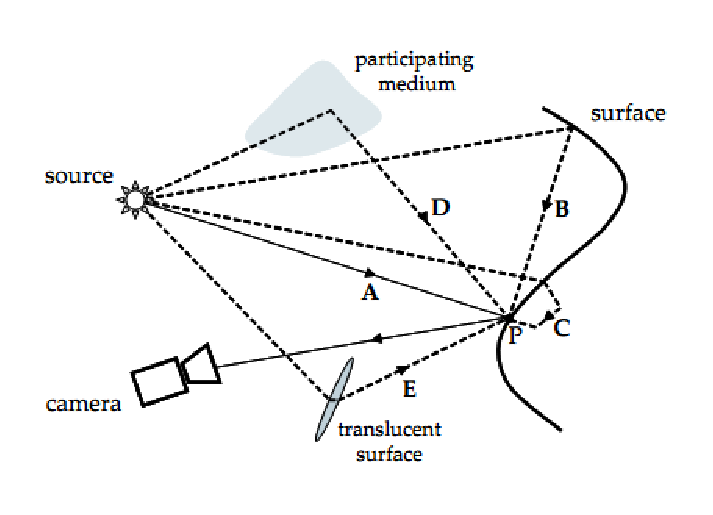
\includegraphics[height=2.5in,width=3.6in]{sep_images/sep2.eps}
%\label{fig:subfig23} } \caption[] {Components of a sponge image: a) Original image, b) Direct c) Global
%component.} 
\label{fig:15} \caption{The luminance of scene point is due to direct illumination
of the point by the source (A) and global illumination due to other
points in the scene which is mainly due to inter-reflections (B), subsurface scattering (C), volumetric scattering (D)
and translucency (E) 
}
\end{figure*}

\begin{figure*}[t]
\centering
\subfigure[$l_u=.61$,$l_v=.35$]{
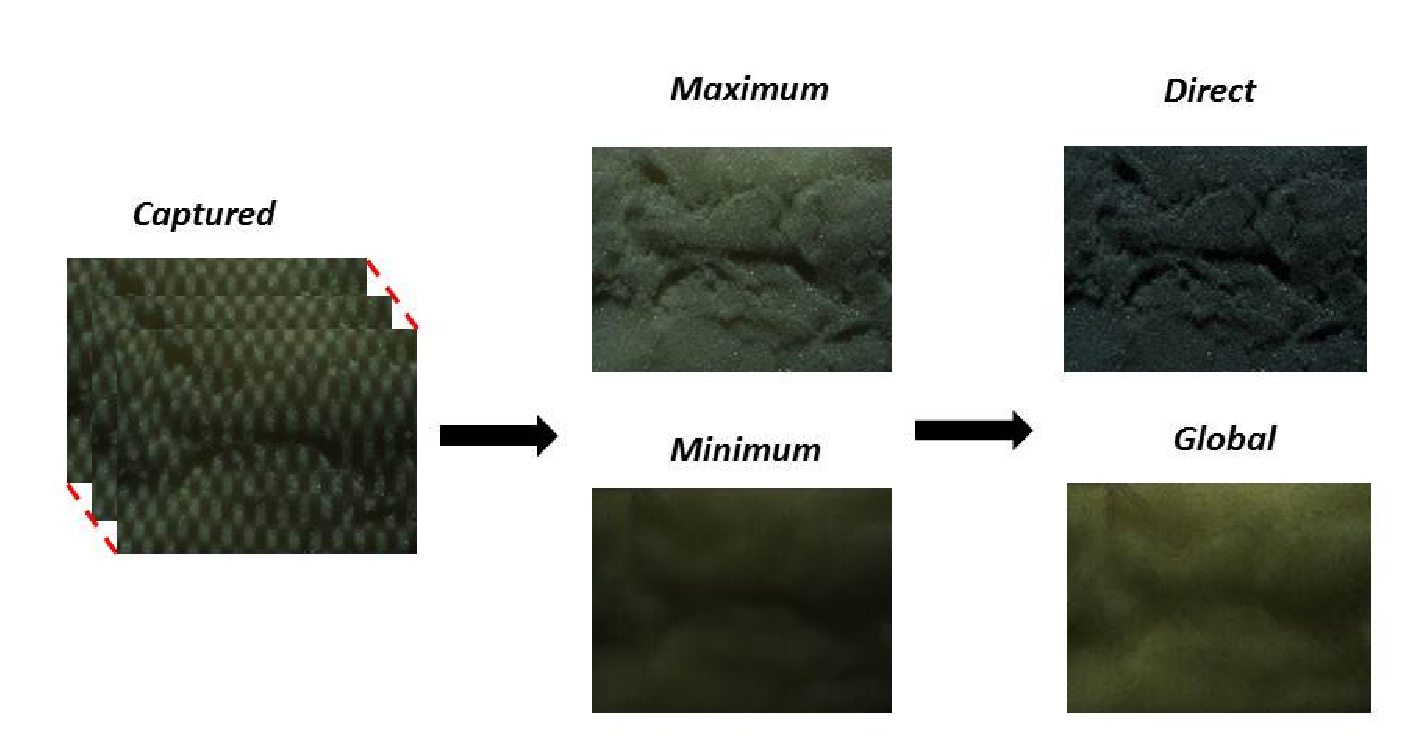
\includegraphics[scale=.46]{sep_images/sep1.eps}
\label{fig:subfig1}
}
%\subfigure[Interpolated]{
%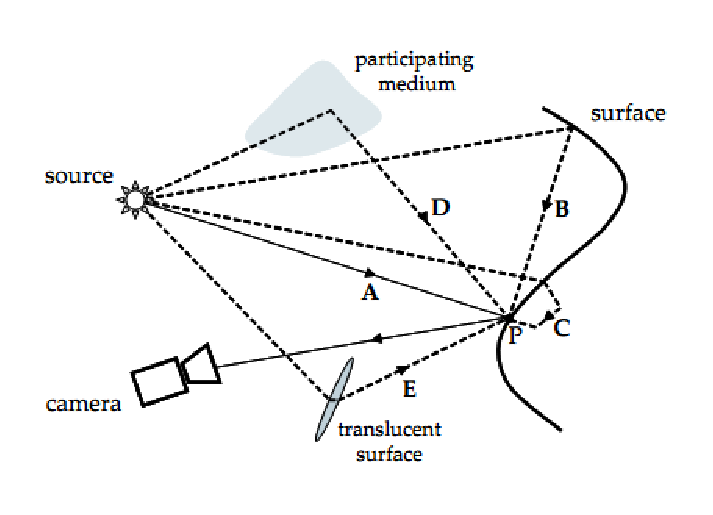
\includegraphics[scale=.26]{sep_images/sep2.eps}
%\label{fig:subfig2}
%}
\caption{The steps involved in the computation of direct and
global images using a set of shifted checkerboard illumination patterns}\label{fig:16}
\end{figure*}

%The luminane of a surface point measured by the camera due to such a scattering event is referred to as the direct
%component.

%The remaining radiance measured by the camera pixel is referred to
%as the global component, Lg. In computer graphics, this term is typically used to denote interreflections – light received by a surface
%point after reflection by other scene points. Here, we are using a
%more general definition. In addition to interreflections, the global illumination received by the surface point may be due to volumetric
%scattering, subsurface scattering or even light diffusion by translucent surfaces.

%In all cases, the totalradiance measured at a camera pixel is the sum
%of the direct and global components:
%L=Ld +Lg 

%Due to light leakages within the projector optics and cus-
%tom image processing incorporated by the manufacturer, the lit and
%unlit checkers have brightness variations within them. Furthermore,
%due to the limited depth of field of the projector, the checkers can
%be defocused in some scene regions

In our experiments, we used checkerboard pattern that were 10x10 pixels in
size and was shifted by 5 times (by 3 pixels each time) in each of
the two dimensions to capture a total of 25 images. The separation
step is given in Figure \ref{fig:16}.

% \begin{figure}[t]
% \centering
% \subfigure[Scene]{
% 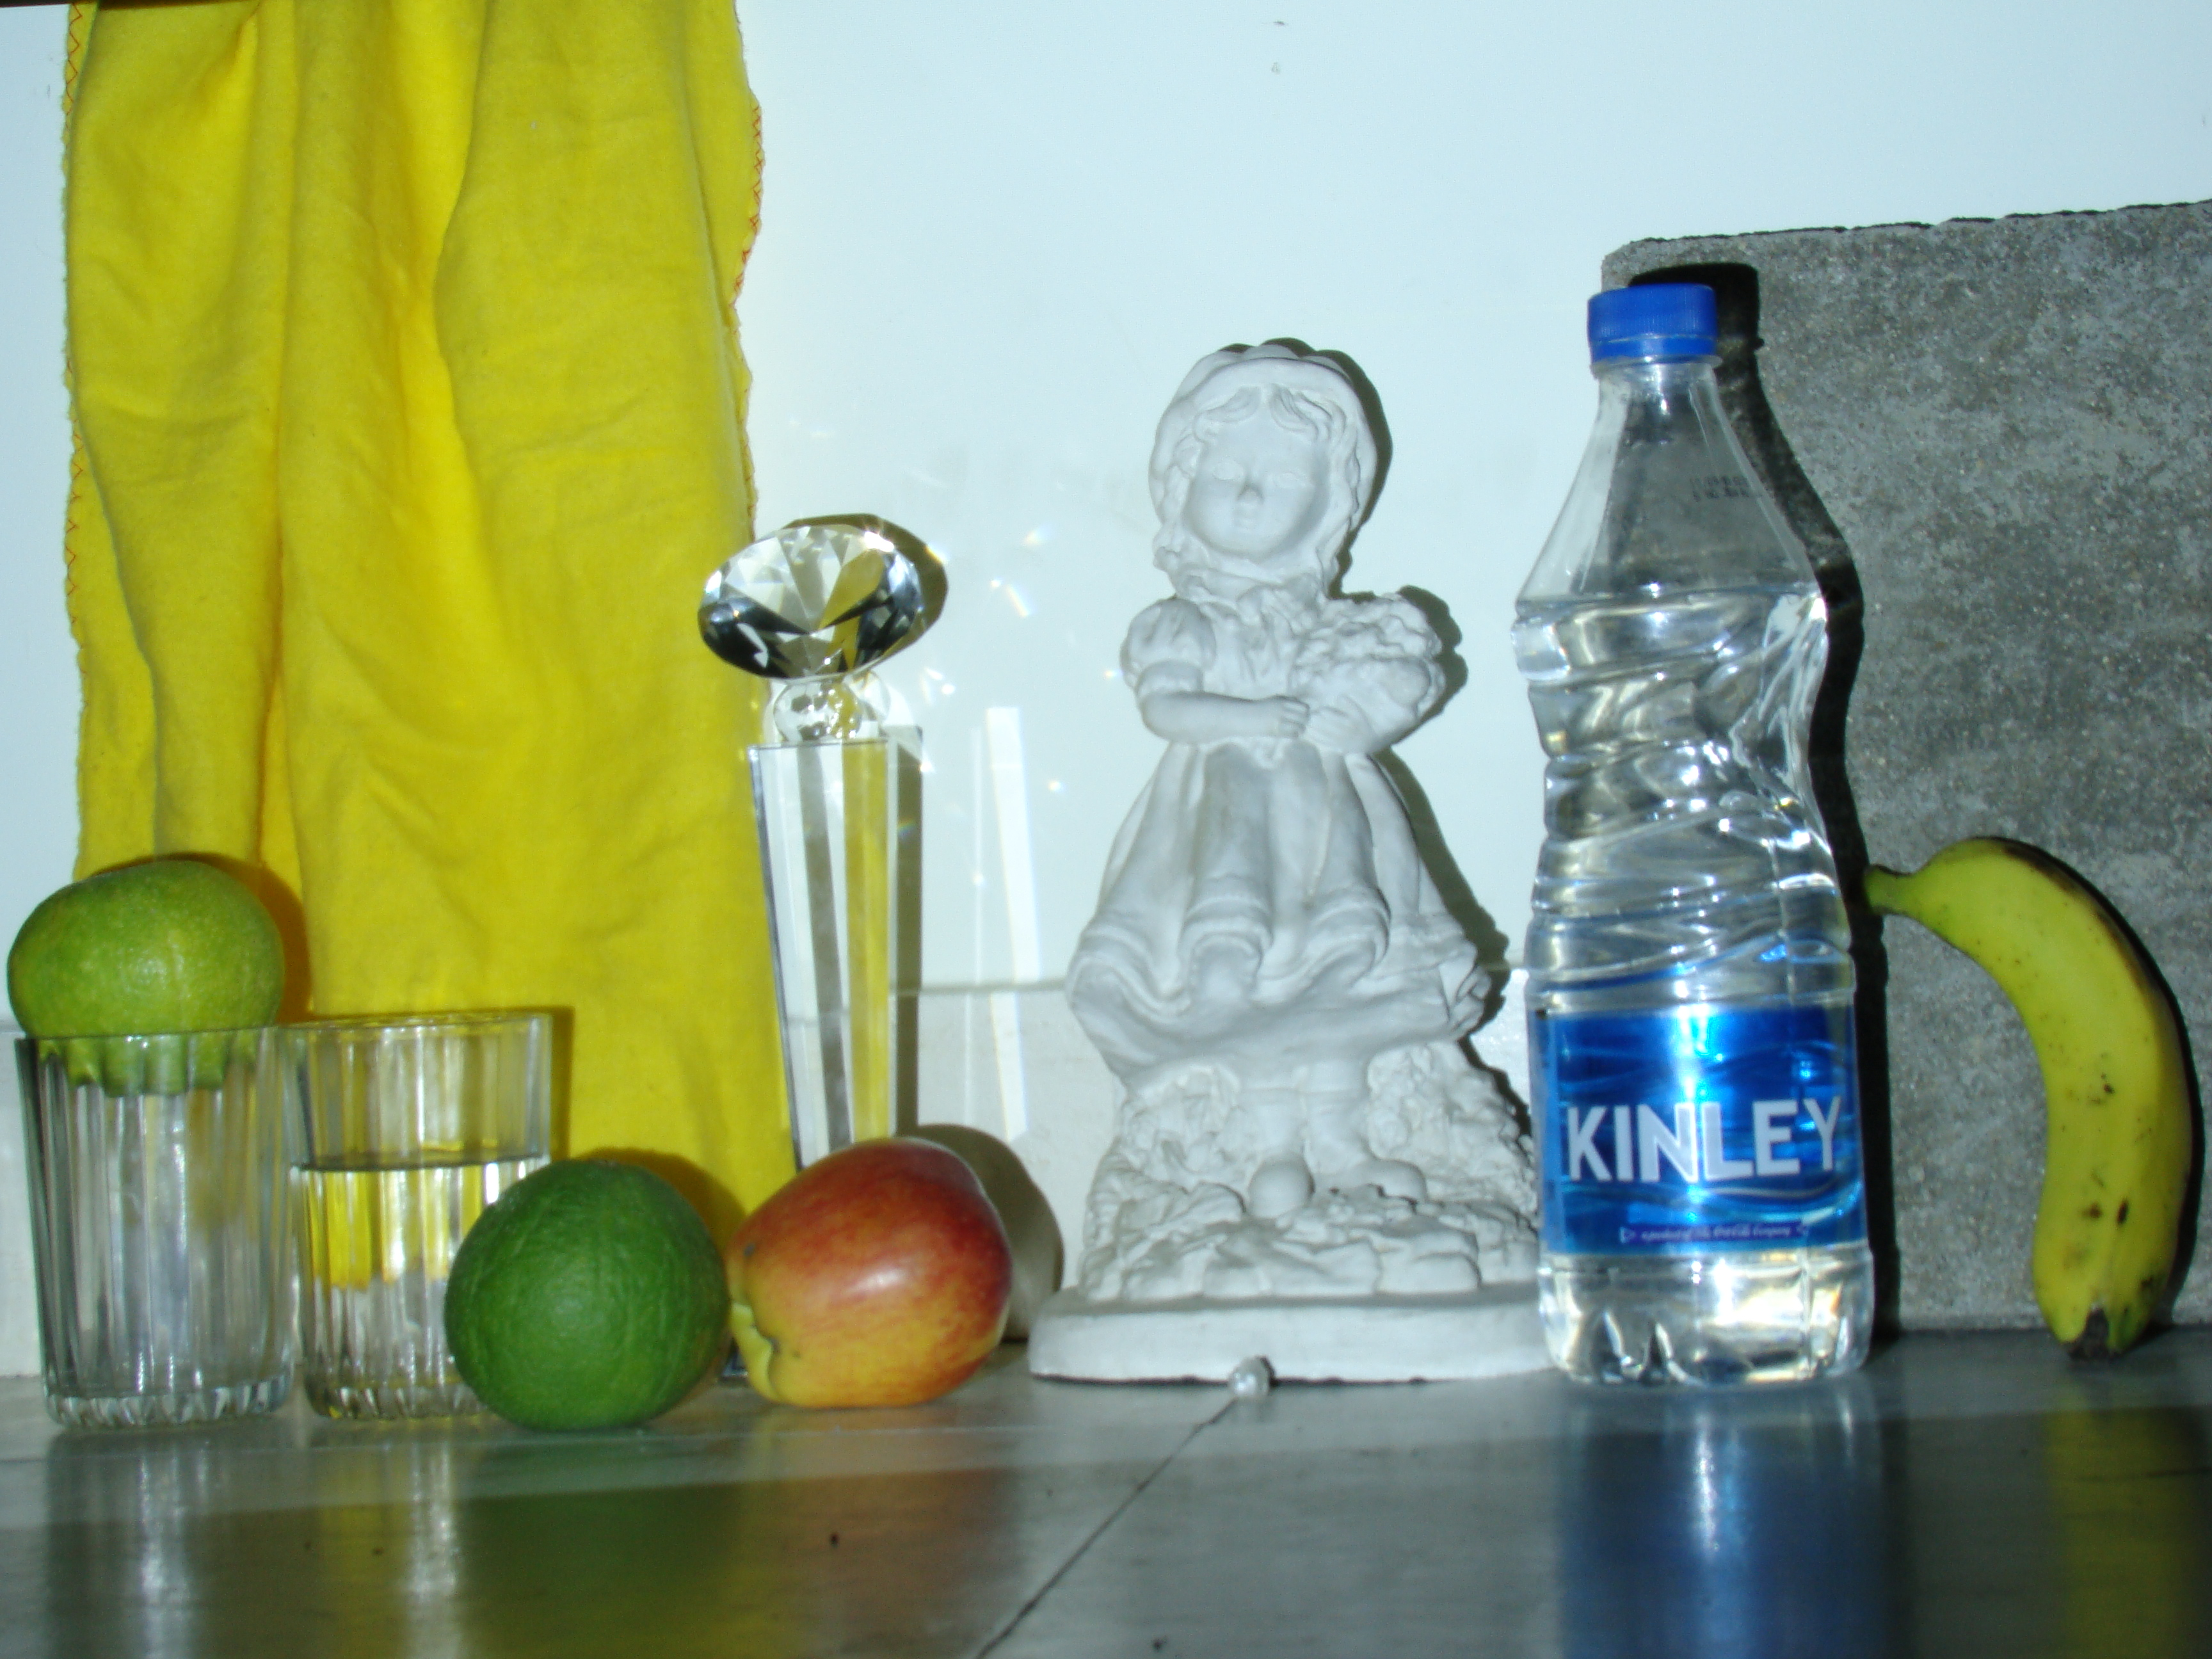
\includegraphics[height=1.2in,width=1.5in]{chap3/res_1/white.eps}
% \label{fig:subfig1}
% }
% \subfigure[Direct Component]{
% 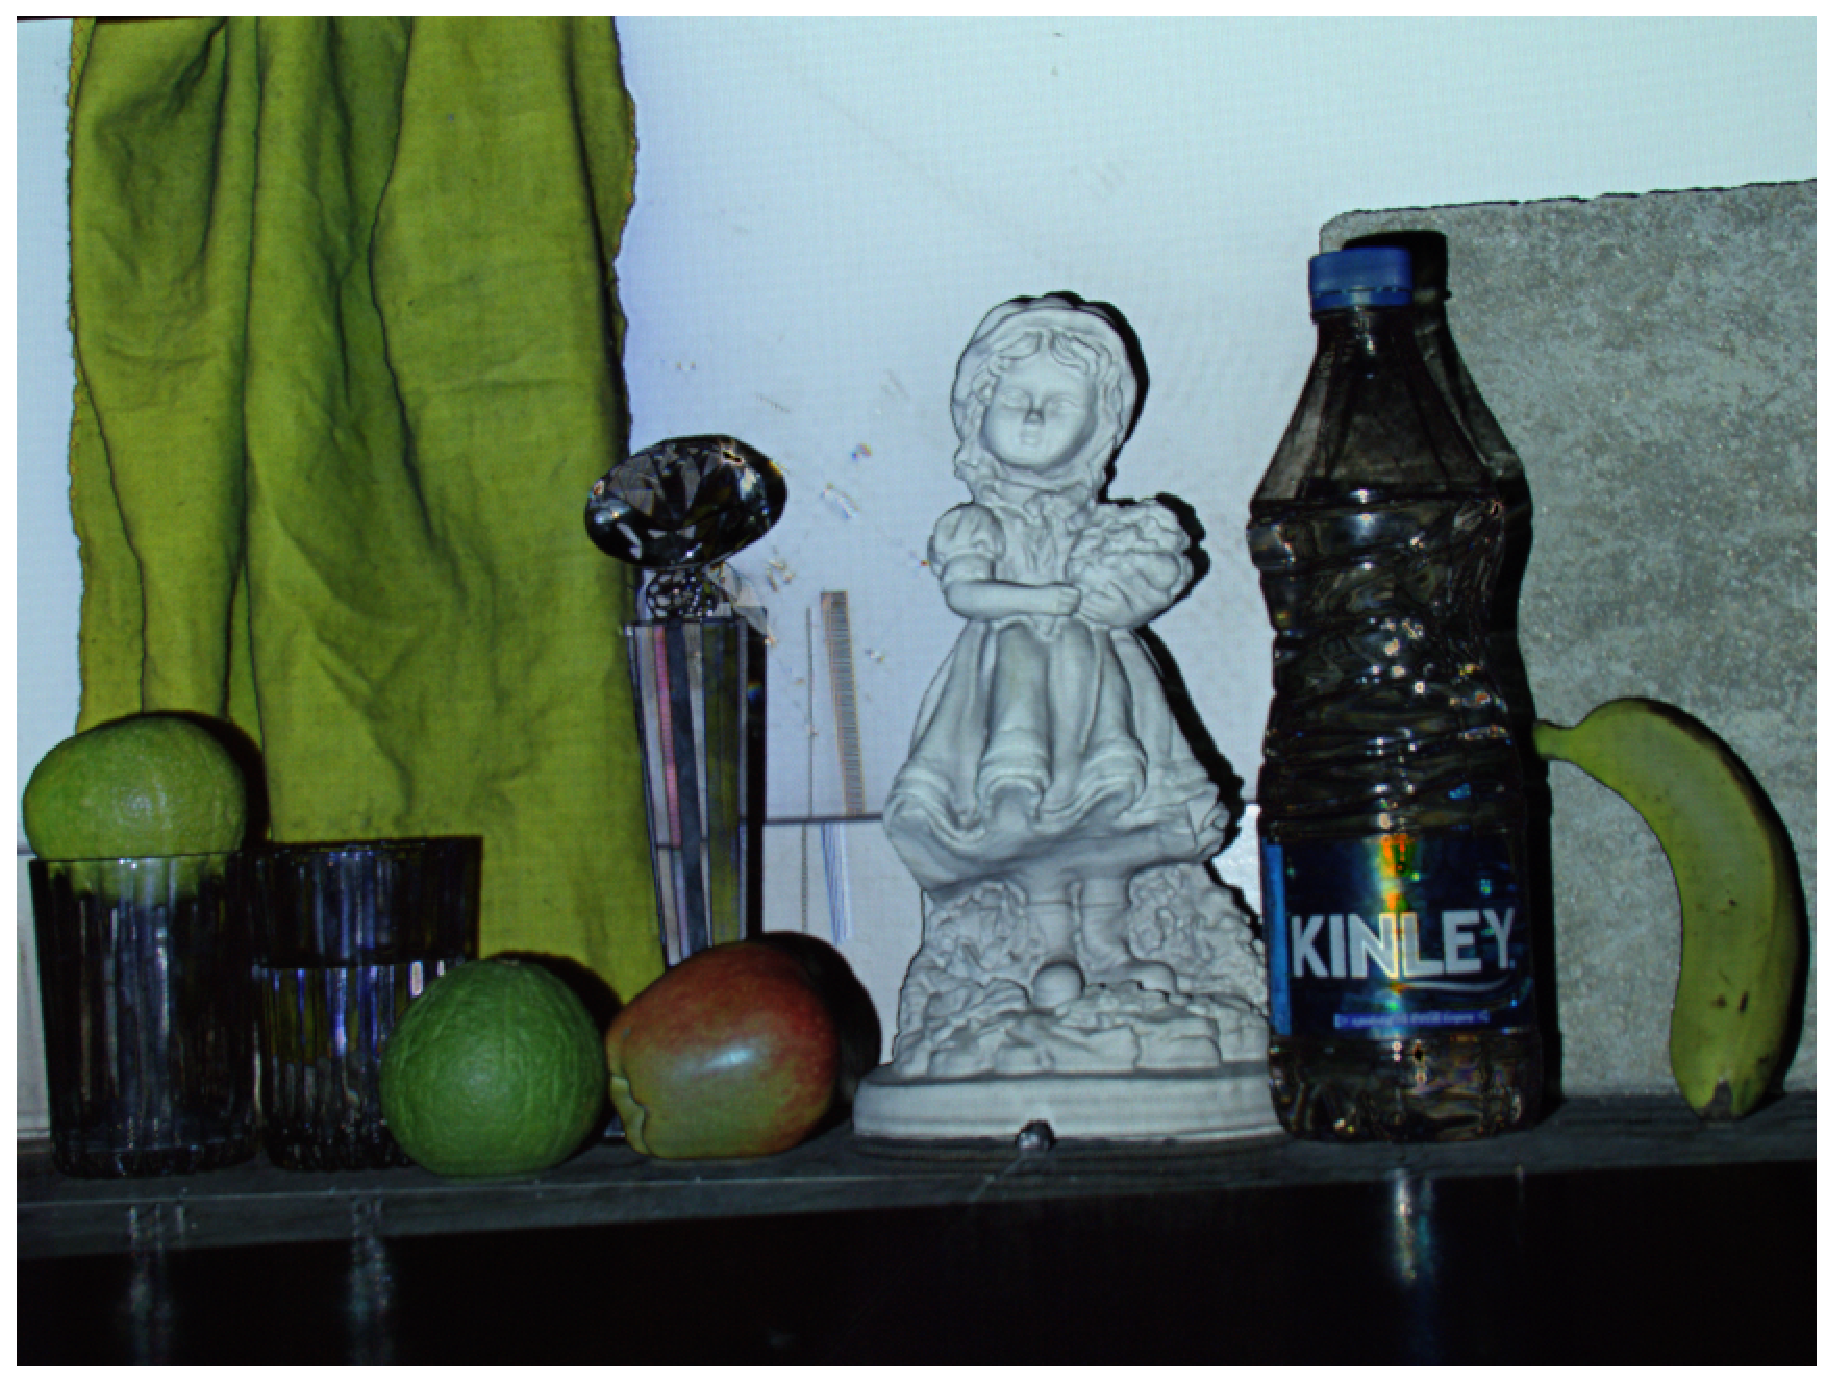
\includegraphics[height=1.2in,width=1.5in]{chap3/res_1/directImg.eps}
% \label{fig:subfig2}
% }
% \subfigure[Global Component]{
% 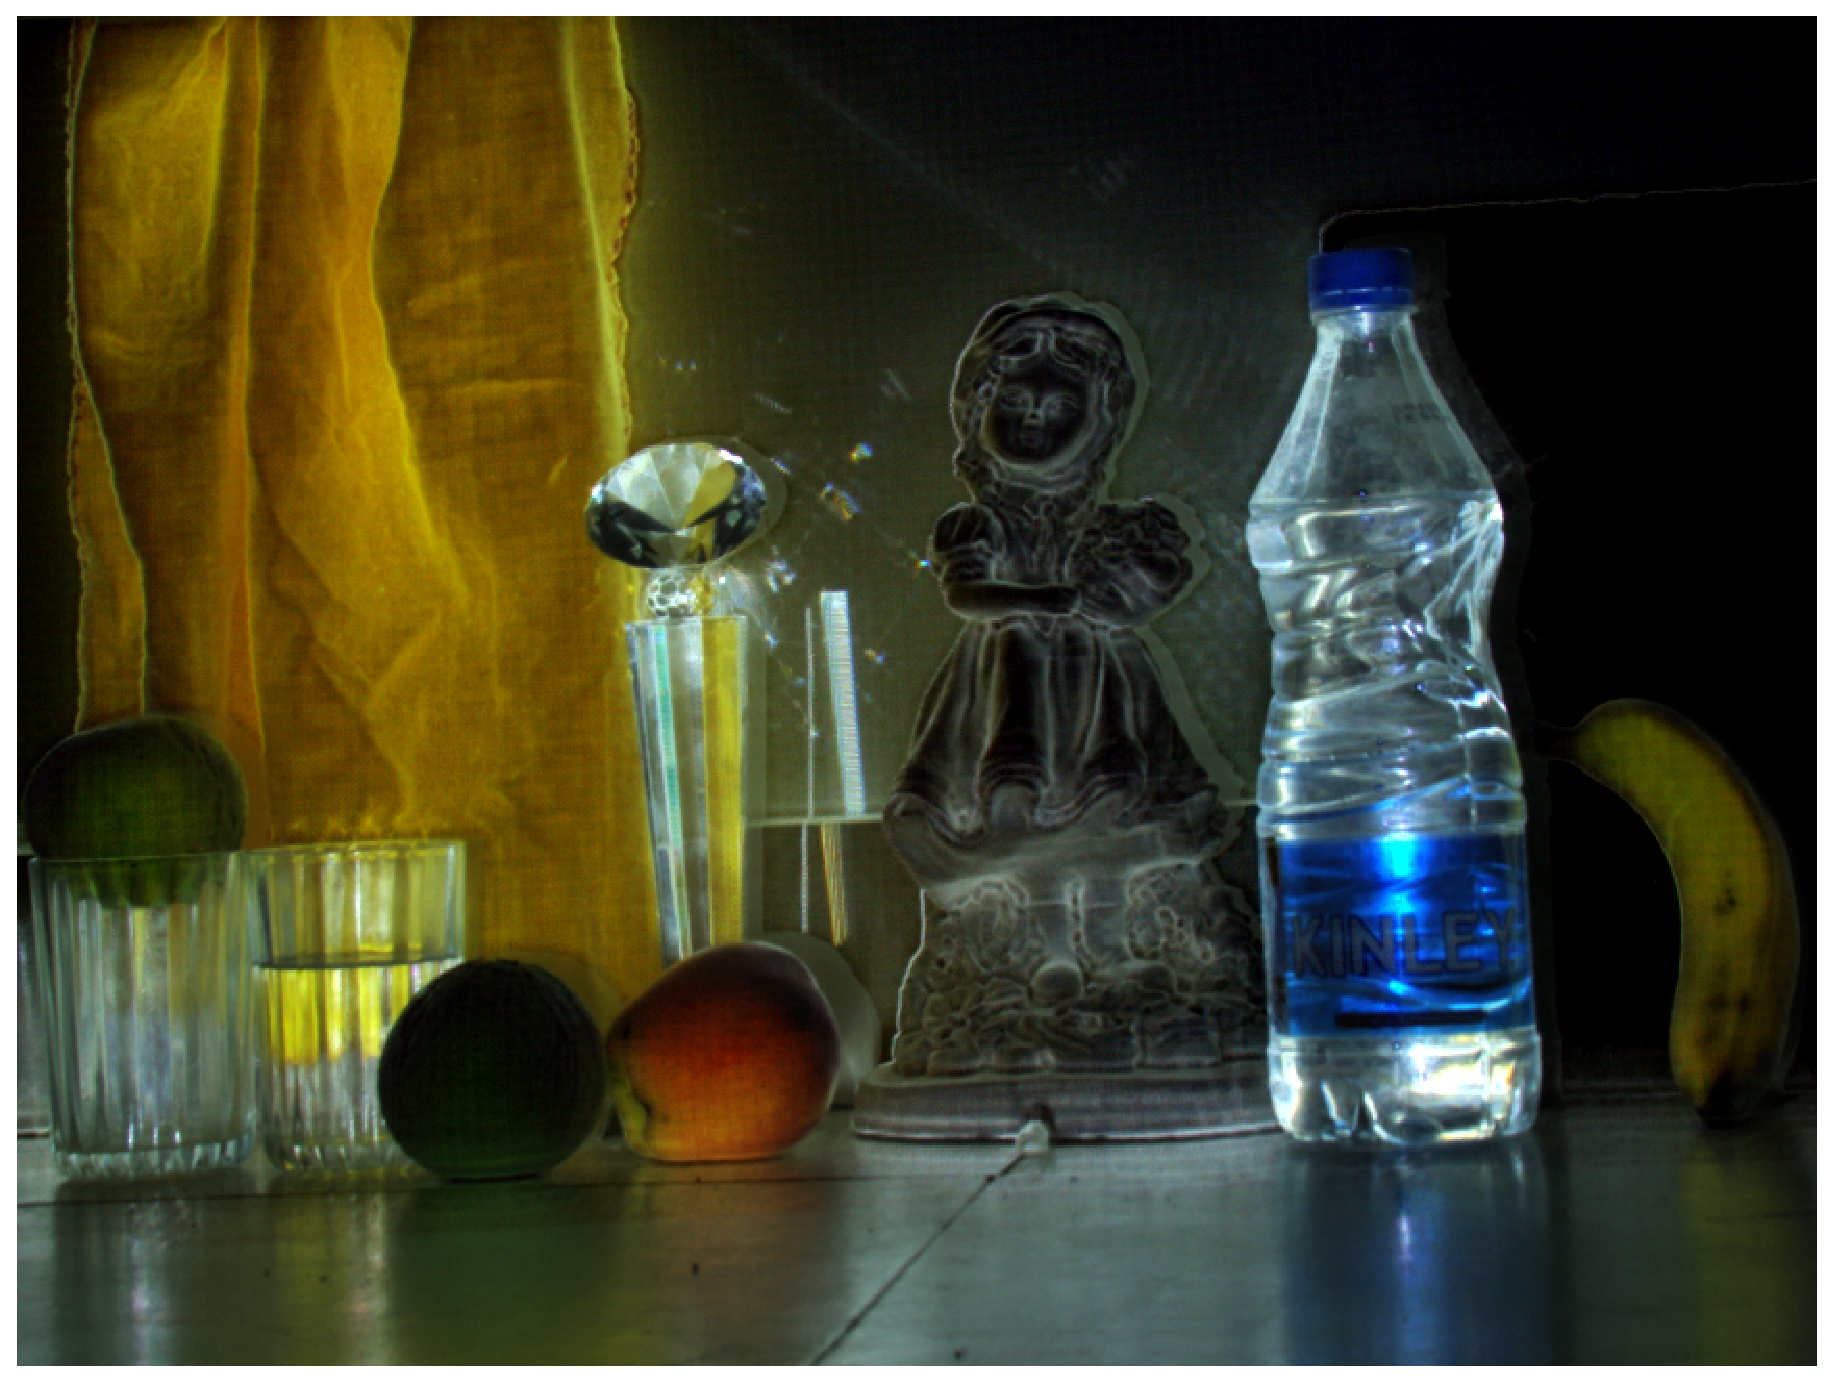
\includegraphics[height=1.2in,width=1.5in]{chap3/res_1/globalImg.eps}
% \label{fig:subfig3}
% }
% \caption{Separation result of a scene}  \label{fig:intExample}
% \end{figure}

\begin{figure*}[t]
\centering
\subfigure[$l_u=.61$,$l_v=.35$]{
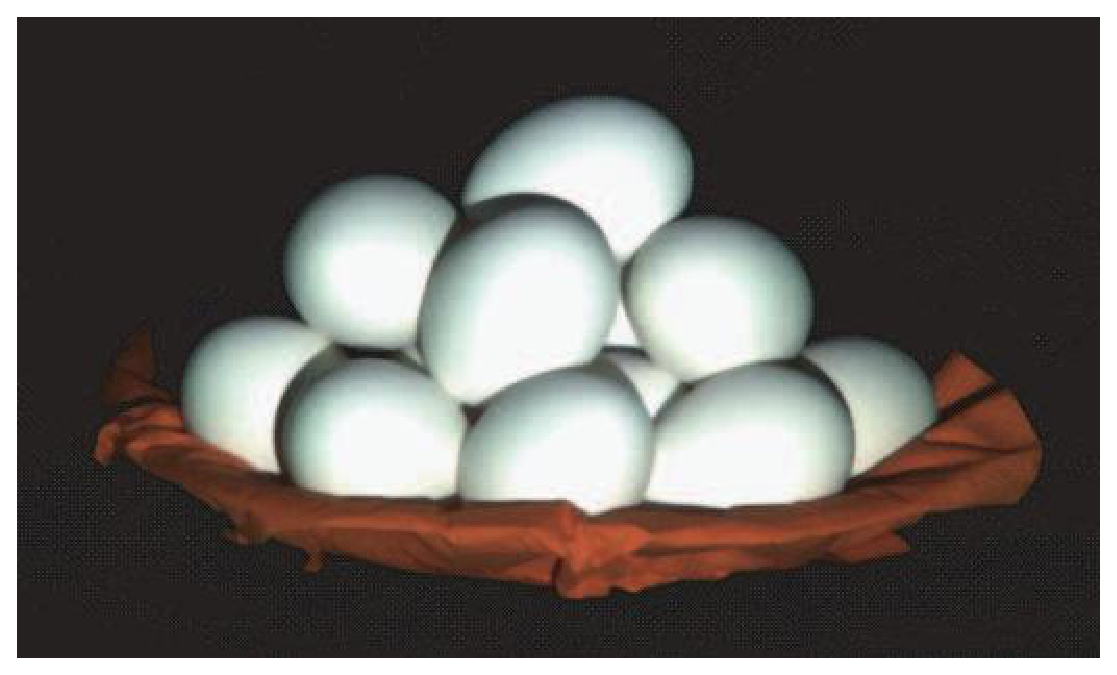
\includegraphics[scale=.26]{images/r1.eps}
\label{fig:subfig1}
}
\subfigure[Interpolated]{
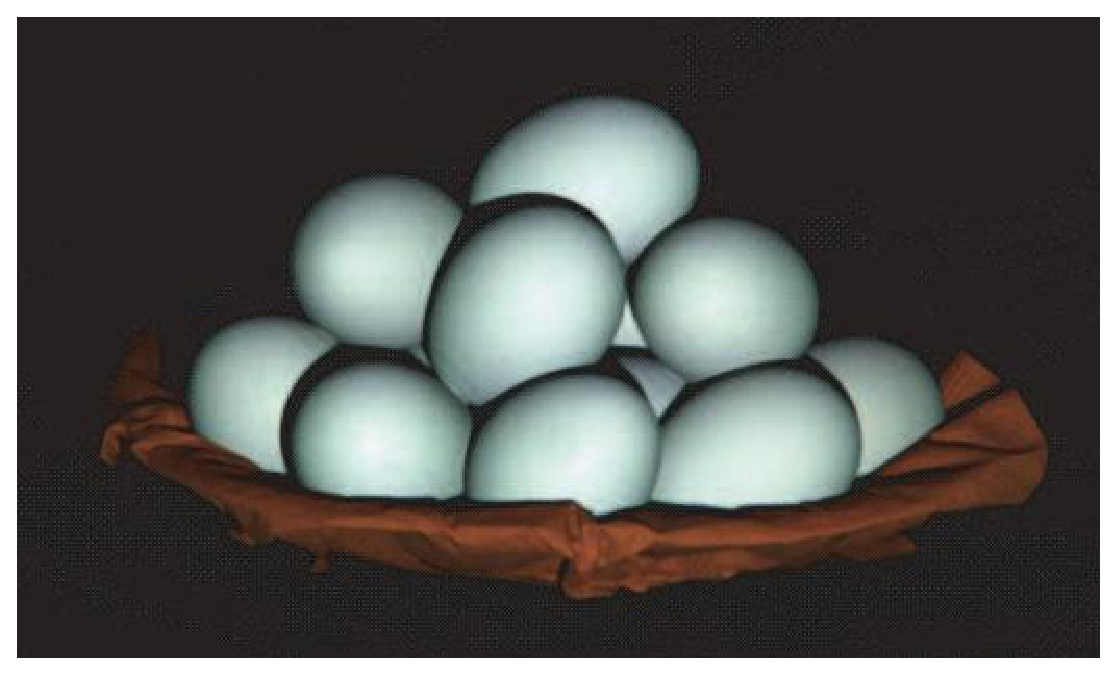
\includegraphics[scale=.26]{images/r2.eps}
\label{fig:subfig2}
}
\subfigure[$l_u=-.61$,$l_v=-.35$]{
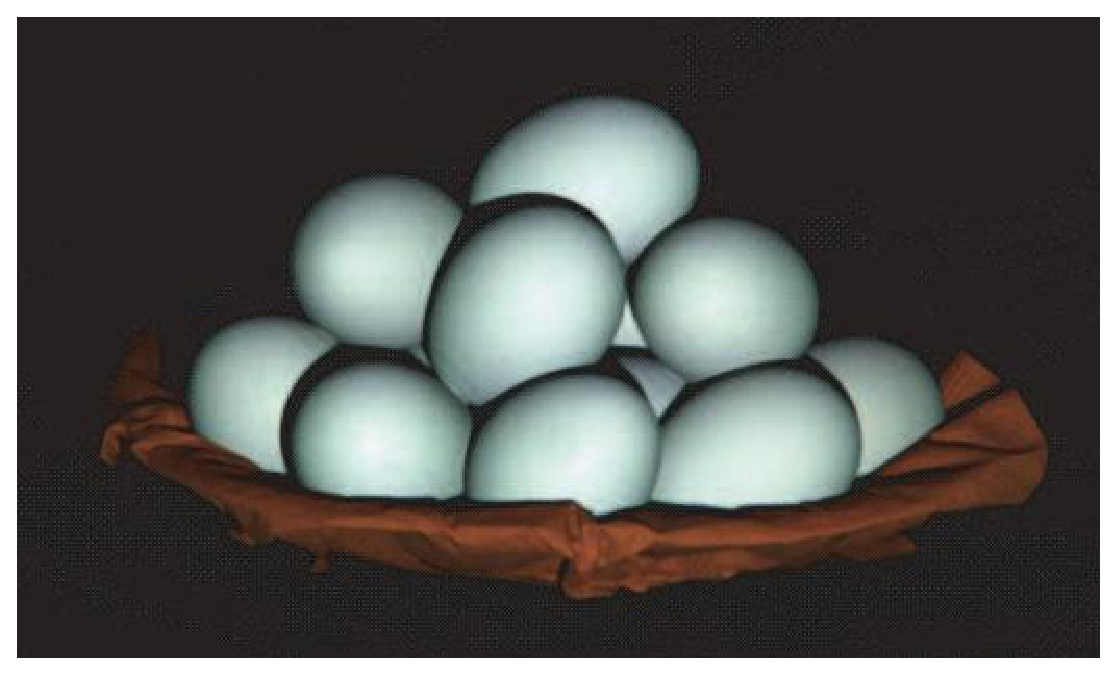
\includegraphics[scale=.26]{images/r3.eps}
\label{fig:subfig3}
}
\subfigure[$l_u=.86$,$l_v=0$]{
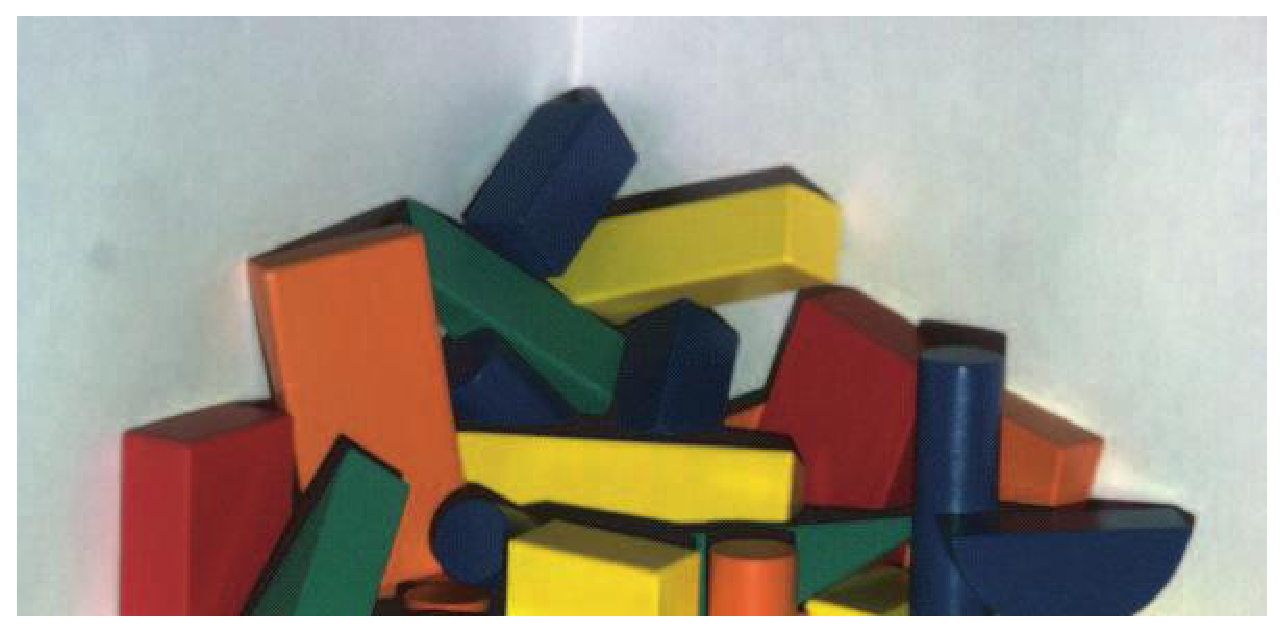
\includegraphics[scale=.23]{images/r4.eps}
\label{fig:subfig1}
}
\subfigure[Interpolated]{
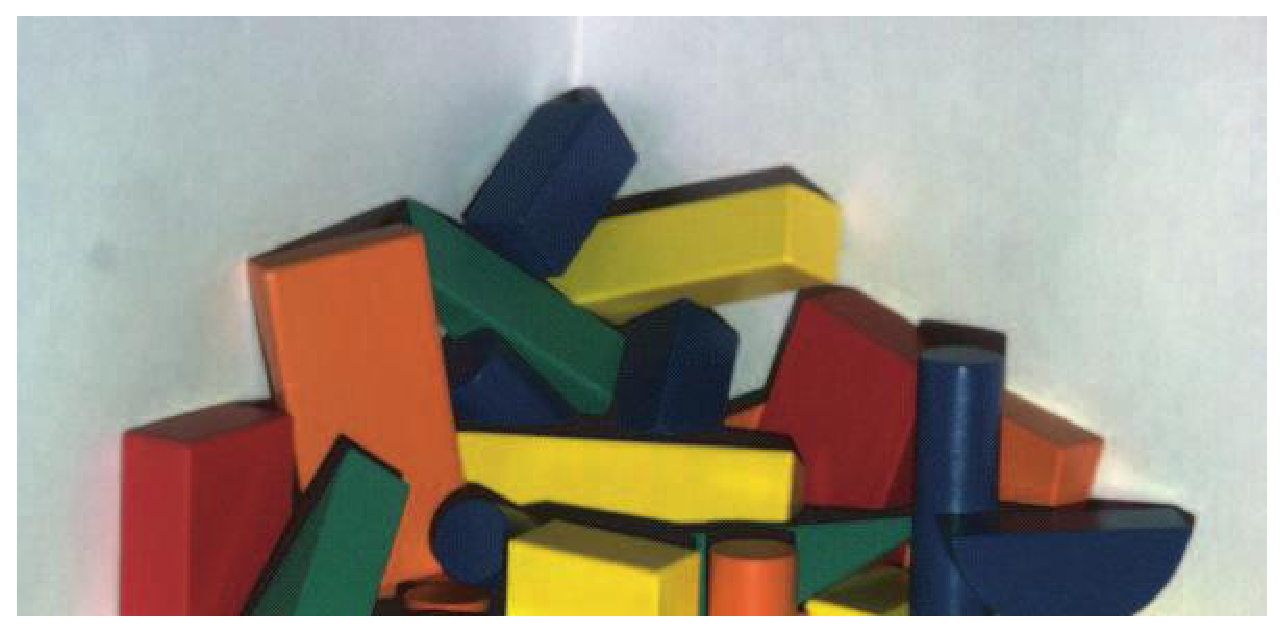
\includegraphics[scale=.23]{images/r5.eps}
\label{fig:subfig2}
}
\subfigure[$l_u=.58$,$l_v=0$]{
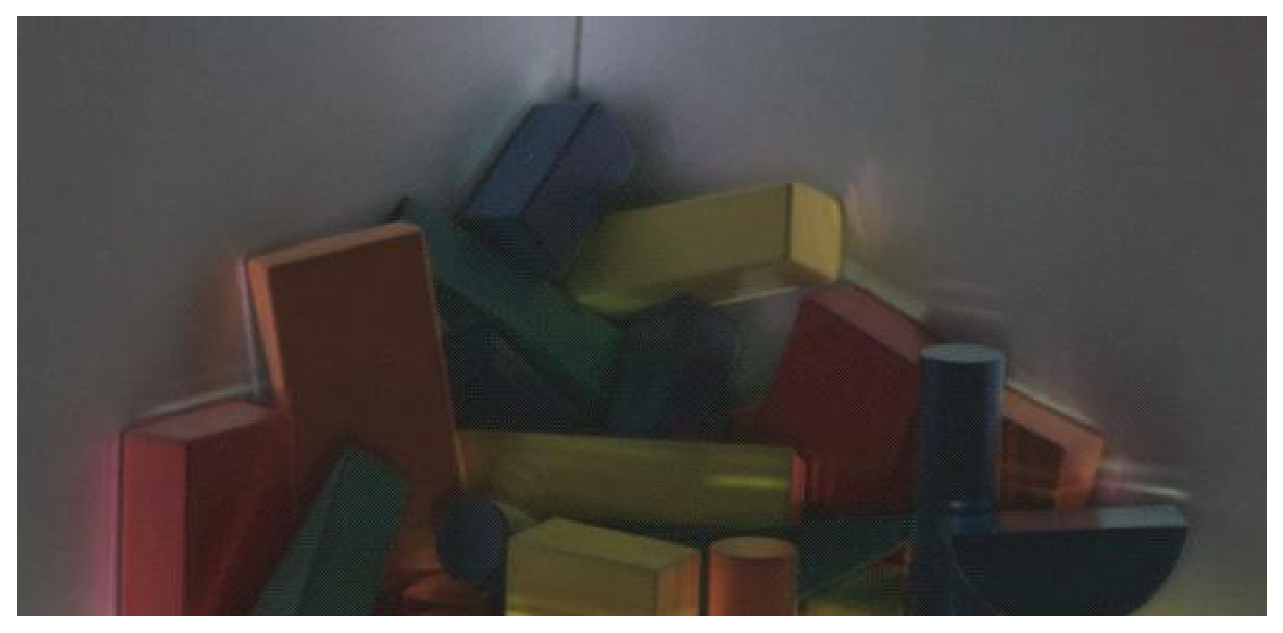
\includegraphics[scale=.23]{images/r6.eps}
\label{fig:subfig3} }
\caption{Shadow interpolation in two directions: a,c) images with horizontally
varying lighting directions, b) interpolated direct image between the two; d,f)
images with vertically varying lighting directions, e) interpolated direct image
between the two.}  \label{fig:intExample}
\end{figure*}
%Figure 2 shows the direct and global component of a cloth piece.

If we separate the image of the texture into direct and the global part, we find
that the shadows and the specularities appear very strongly in the direct part,
as these are phenomena that involve light that reaches the surface point
directly from the light source. The fine details and the structure of the
material are very prominently visible in the direct part as they are observed
primarily through shadows. On changing the lighting direction, the change in the
luminance of the direct part is minimal as long as the surface point is directly
illuminated. The variations are introduced, primarily by self-shadowing and
specularity, both of which are abrupt changes as the lighting direction changes.
The global component contains the the lighting of a surface point from other
parts in a scene, and hence the captures the overall illumination as well as
color variations of a surface with lighting direction. As the lighting direction
changes, the luminance value of the global part varies significantly.

Both direct and global components are separately analyzed to derive the
corresponding models and parameters. Given a new lighting direction, we use the
two models separately to generate the corresponding components, and combine them
to get the final image.Then for a new lighting direction, we can readily
interpolate both specular content as well as shadows.
% In our method, we analyze each of these phenomena separately and capture the
% results using appropriate models. We first separate the images into two
% components: One is the {\em direct} part,which captures the light that is
% directly reflected by the surface point from the source and other is the {\em global} part which
% is due to the illumination of the point from all other points of the scene. Separation of a scene
% into global and direct part can be done by illuminating the scene with a high
% frequency binary pattern \cite{A9}. 
% Fig. \ref{fig:figure2} shows the direct and global component of sponge texture.
% 
% The shadows and the specularities appear very strongly in the direct part,
% as these are phenomena that involve light that reaches the surface point
% directly from the light source. The fine details and the structure of the
% material are also very prominently visible in the direct part.
% The global component contains the lighting of a surface point from other
% parts in a scene, and hence captures the overall illumination as well as
% color variations of a surface with lighting direction.

\begin{figure}[t]
\centering
\subfigure{
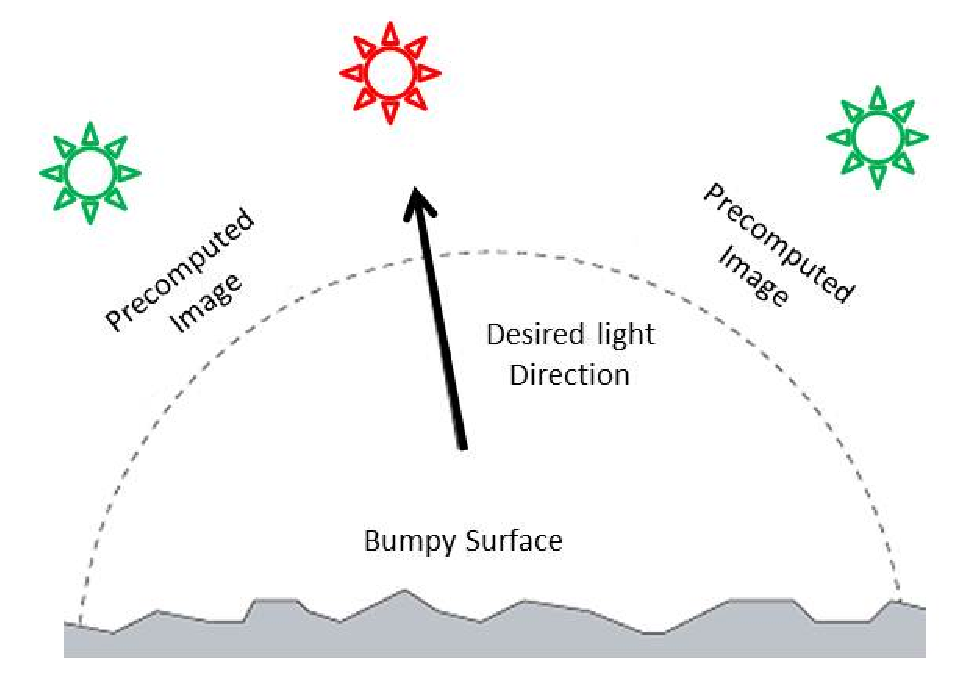
\includegraphics[scale=.52]{chap3/res_2/inter.eps}
\label{fig:subfig1}
}
\caption{shadow modeling by interpolation}
\end{figure}
\begin{center}
\begin{figure*}[t]
\centering
\subfigure[]{
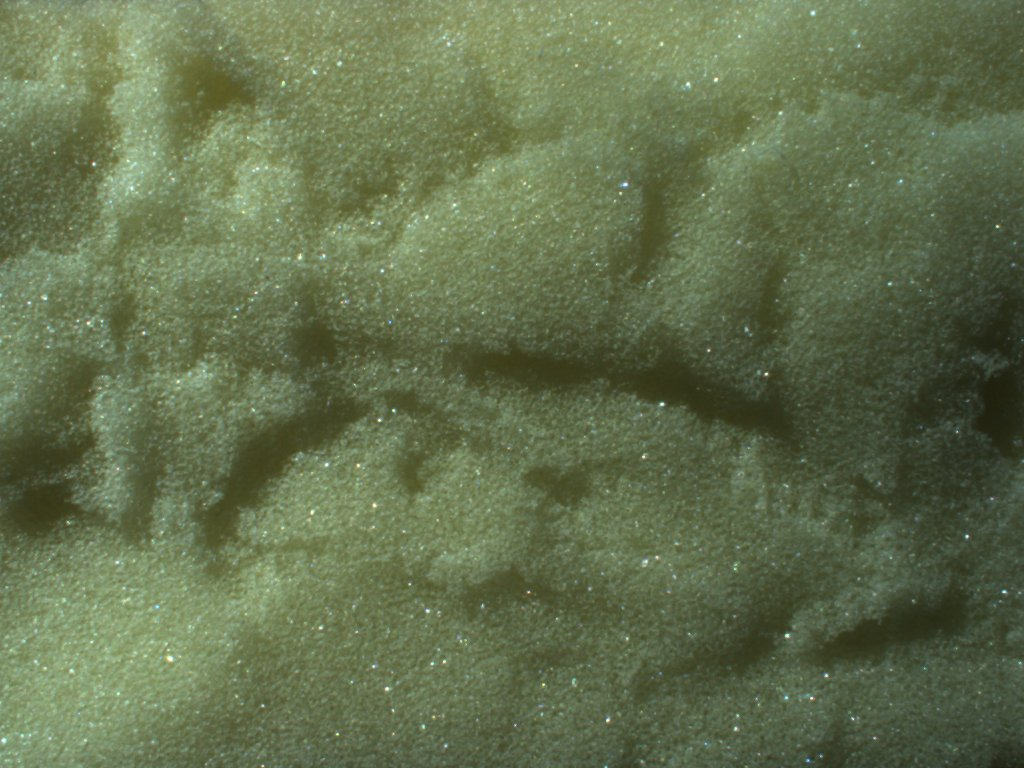
\includegraphics[scale=.139]{image_eps/direct+global/cloth/orig_30.eps}
\label{fig:subfig1}
}
\subfigure[]{
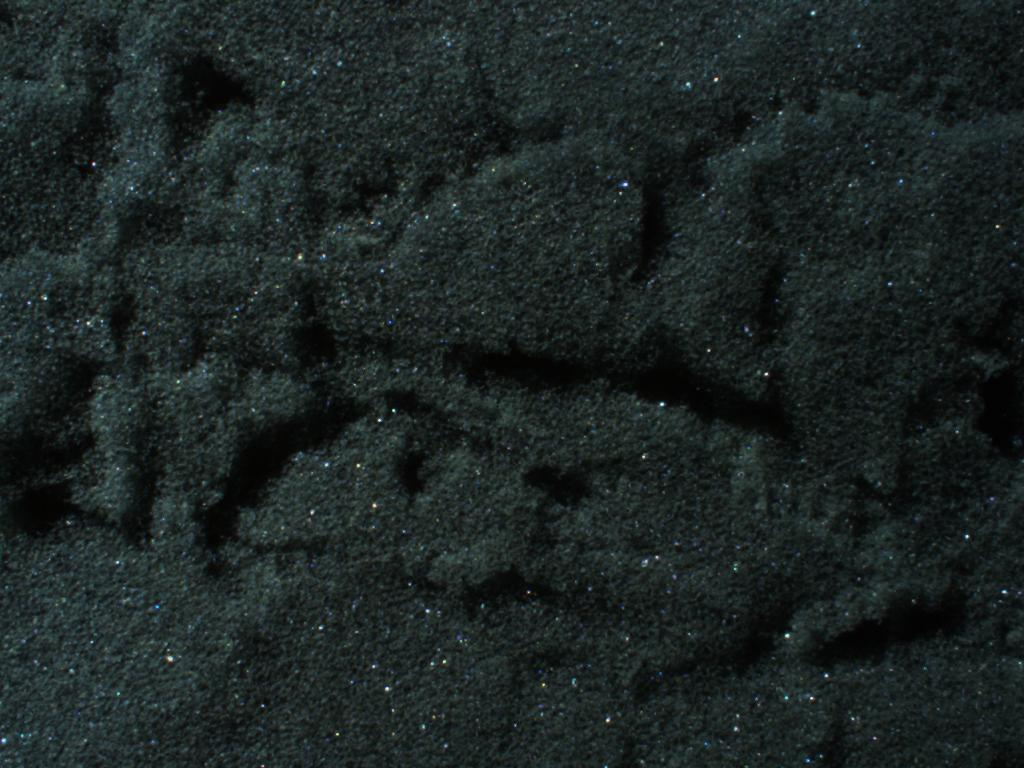
\includegraphics[scale=.139]{image_eps/direct+global/cloth/direct_30.eps}
\label{fig:subfig2}
}
\subfigure[]{

\includegraphics[scale=.139]{image_eps/direct+global/cloth/global_30.eps}
\label{fig:subfig3} } \caption{Components of a cloth image for a specific
lighting direction: a) original image, b) direct component, c) global
component.} \label{fig:subfigureExample}
\end{figure*}
\end{center}
\section{Modelling Direct Component}

As noted before, the direct component is affected by the phenomena of
self-shadowing and specularity, in addition to the lambertian reflectance of the
surface point. Shadows are the points the receive no direct light from the
primary source. However, their luminance value is not completely zero. This is
because they get some light from the neighboring pixels because of
inter-reflections. However, when the image is decomposed into direct and global
component, the luminance value of shadow region (due to inter-reflections)
appear in global part and thus direct part is left with dark prominent shadow
regions whose value is near to zero (see Figure 2b). These dark shadow regions
can easily be separated out using thresholding.

A major difficulty in lighting interpolation is the realistic generation of
shadows. To compute shadow masks for real scenes, our approach first infers
shadow pixels from the illumination intrinsic image. The intensities in an
illumination intrinsic image represent magnitudes of incident irradiance, so
image areas with low values indicate shadowed regions. A simple thresholding can
be done to separate out the shadow part. A suitable threshold is determined
using Otsu's method~\cite{B9}.


%%%%%%%%%%%%%%%%%FIGURE NO 3  shadow by interpolation %%%%%%%%%%%%%%%
\begin{figure*}[t]
\centering
\subfigure[$l_u=.61$,$l_v=.35$]{
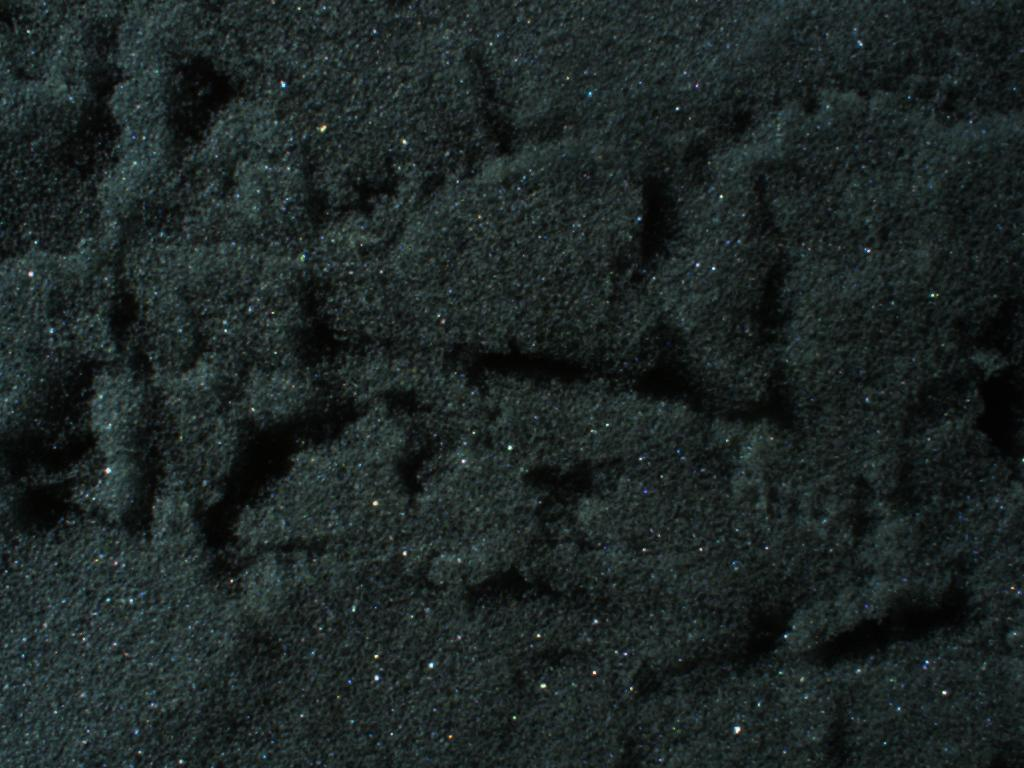
\includegraphics[scale=.12]{image_eps/interpolated/phi=45.eps}
\label{fig:subfig1}
}
\subfigure[Interpolated]{
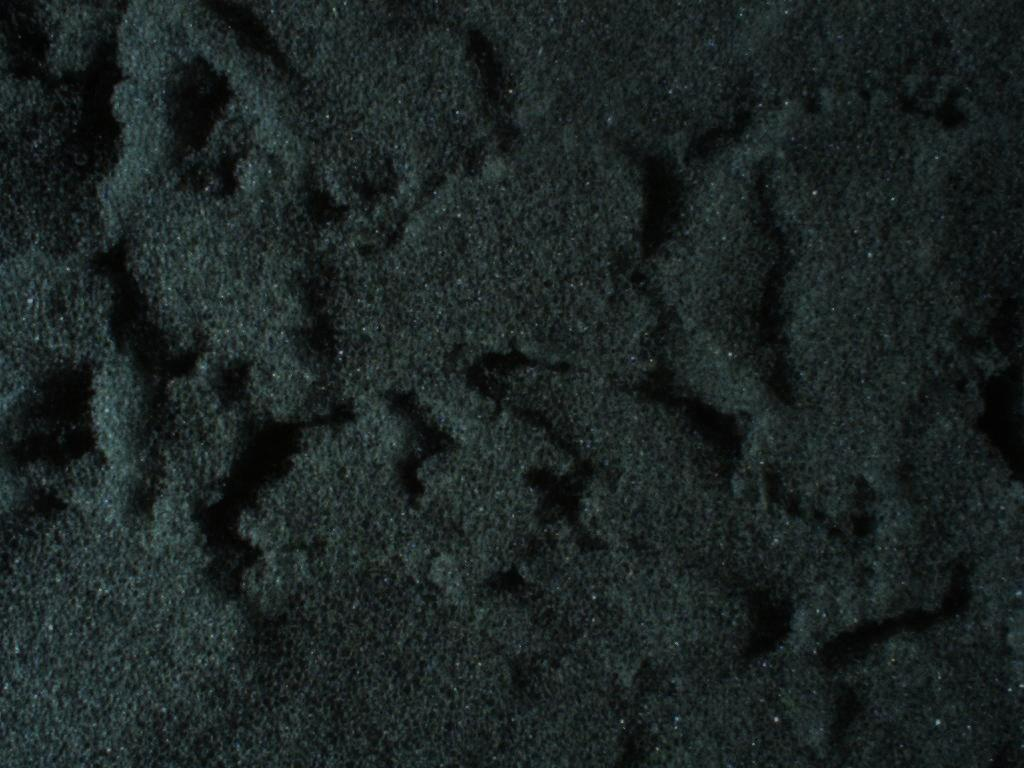
\includegraphics[scale=.12]{image_eps/interpolated/direct_90_interpol.eps}
\label{fig:subfig2}
}
\subfigure[$l_u=-.61$,$l_v=-.35$]{
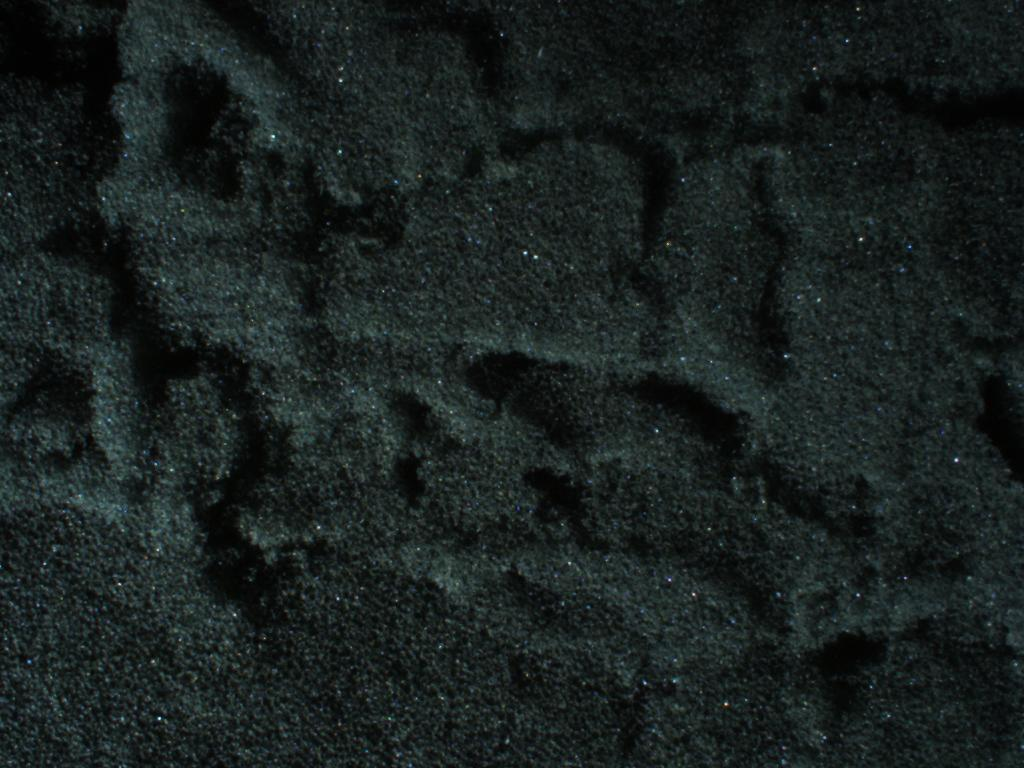
\includegraphics[scale=.12]{image_eps/interpolated/phi=135.eps}
\label{fig:subfig3}
}
\subfigure[$l_u=.86$,$l_v=0$]{
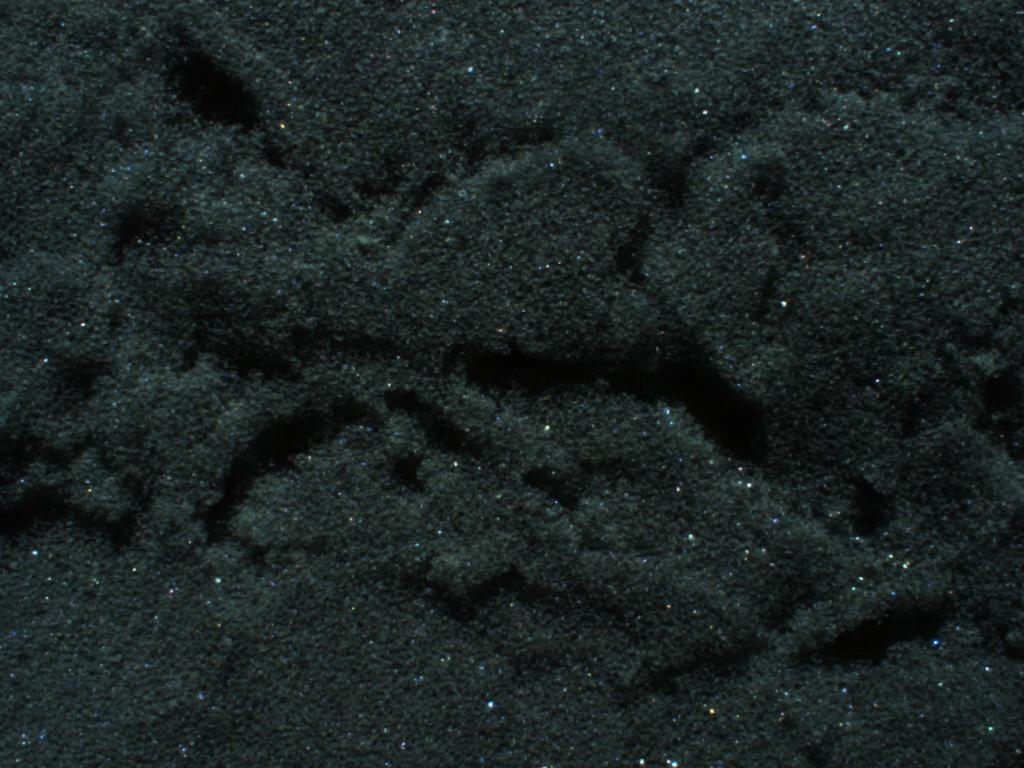
\includegraphics[scale=.12]{image_eps/interpolated/theta=30.eps}
\label{fig:subfig1}
}
\subfigure[Interpolated]{
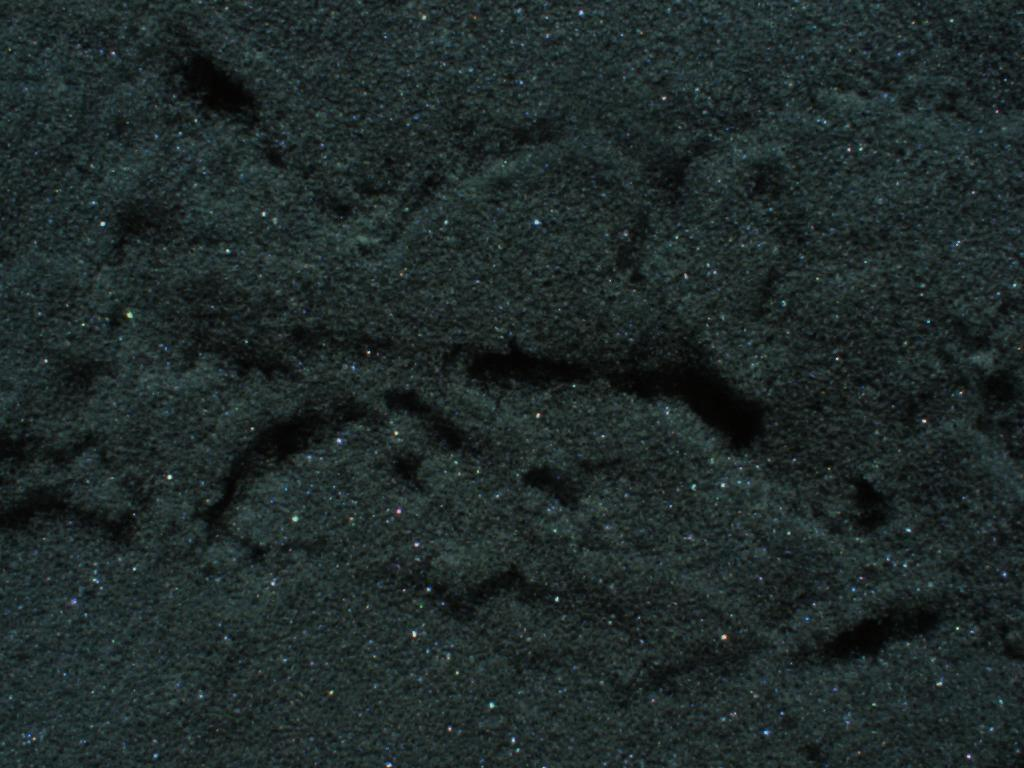
\includegraphics[scale=.12]{image_eps/interpolated/theta=42.eps}
\label{fig:subfig2}
}
\subfigure[$l_u=.58$,$l_v=0$]{
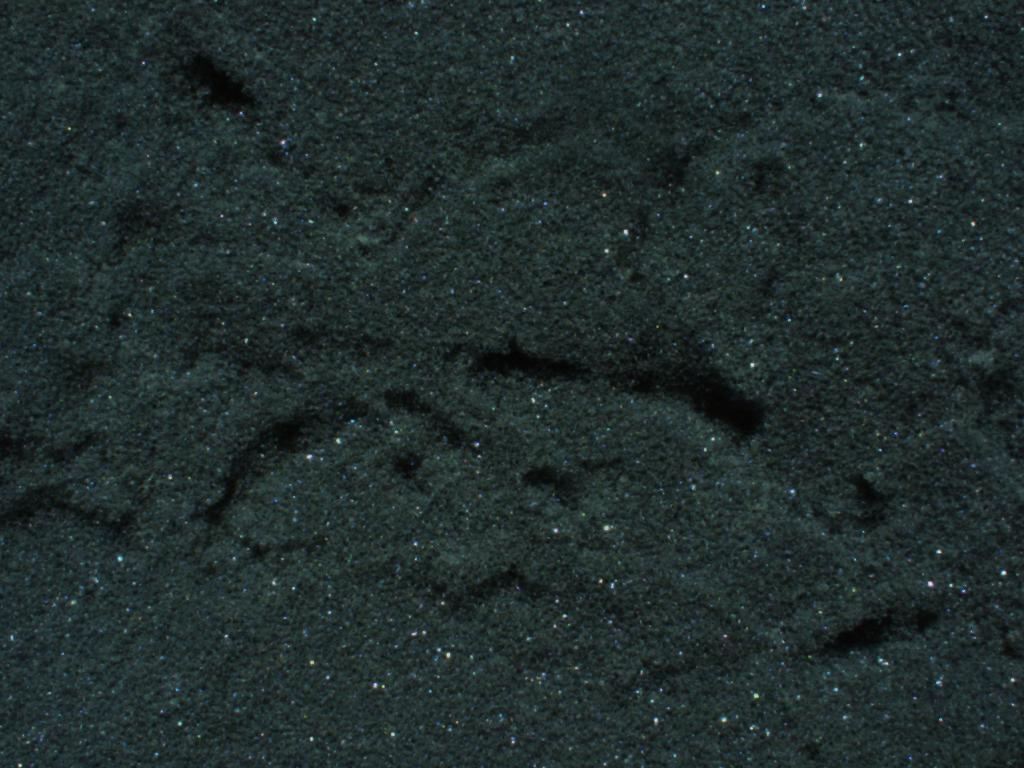
\includegraphics[scale=.12]{image_eps/interpolated/theta=54.eps}
\label{fig:subfig3} }

\caption{Shadow interpolation in two directions: a,c) images with horizontally
varying lighting directions, b) interpolated direct image between the two; d,f)
images with vertically varying lighting directions, e) interpolated direct image
between the two.}  \label{fig:intExample}
\end{figure*}




A variety of shadow detection techniques have been proposed in the past to
capture this phenomenon in a realistic fashion \cite{B7,B10,B11,B17}. In our
approach, as the direct component receives only light directly from the source,
a simple thresholding is quite effective in addition to being efficient. More
details on various shadow algorithms and their complexities can be found in
\cite{B16}. Once the shadow regions are detected in each of the images, we
proceed to capture the variations of it with lighting direction. We discuss two
distinct approaches for this purpose, each with its own merits and
short-comings, and show how they can be combined to derive a good shadow model.




\begin{figure*}[t]
\centering \subfigure[]{
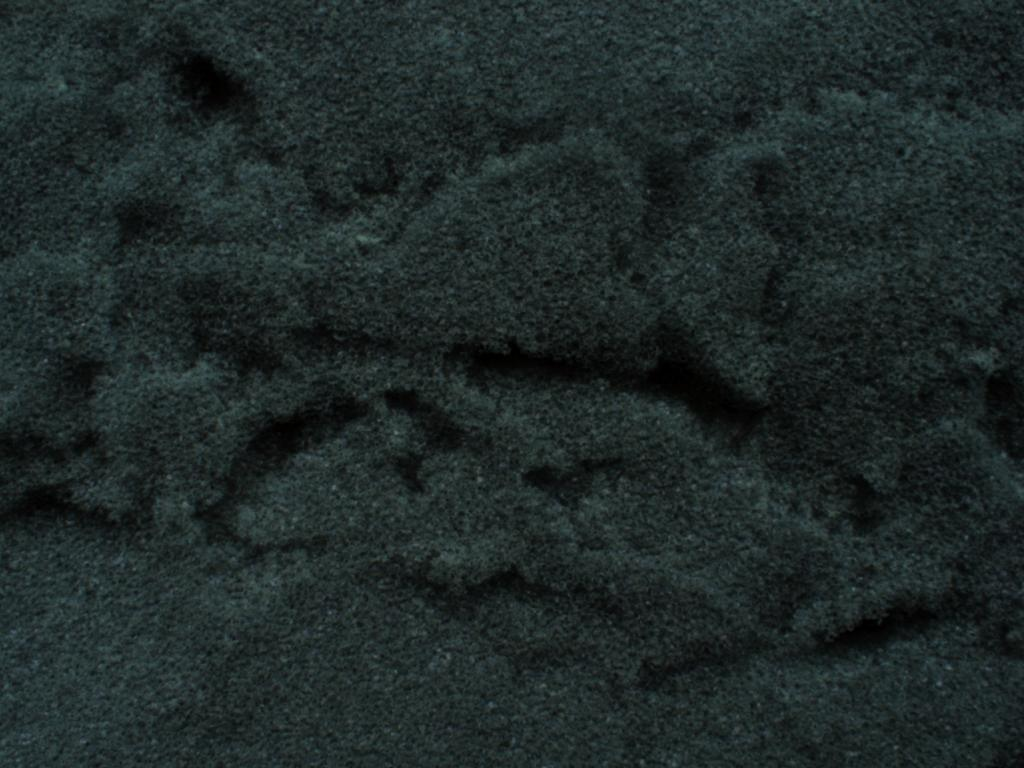
\includegraphics[scale=.12]{image_eps/shadow_classify/linear.eps}
\label{fig:subfig1} } \subfigure[]{
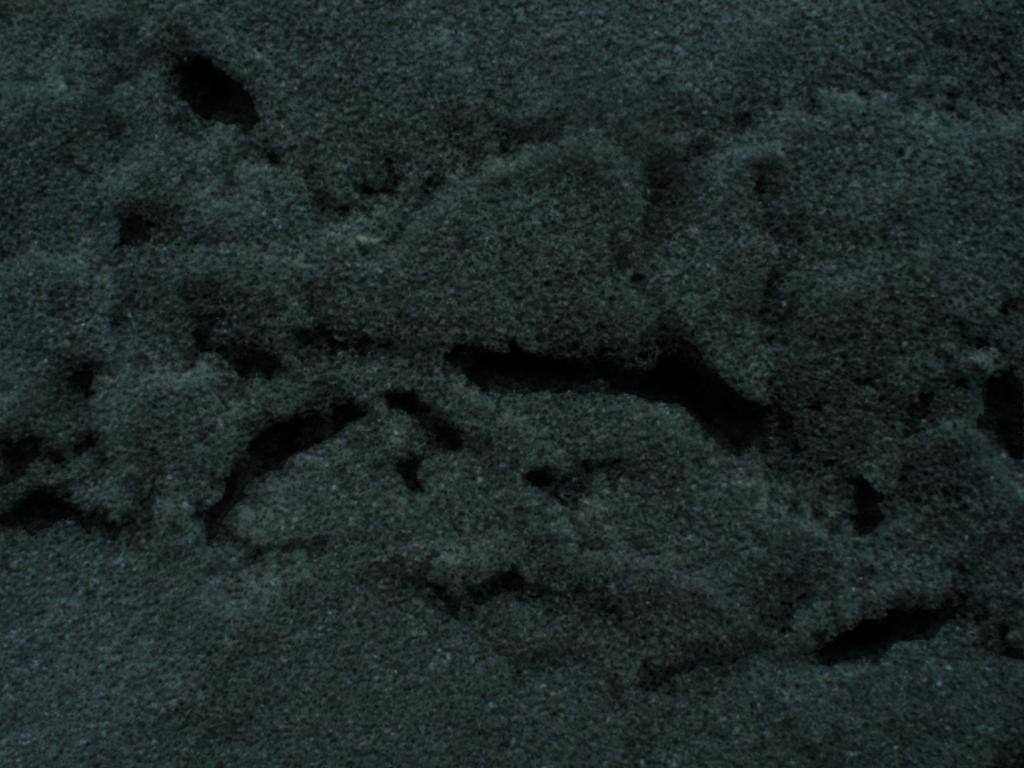
\includegraphics[scale=.12]{image_eps/shadow_classify/shadow.eps}
\label{fig:subfig2} } \subfigure[]{
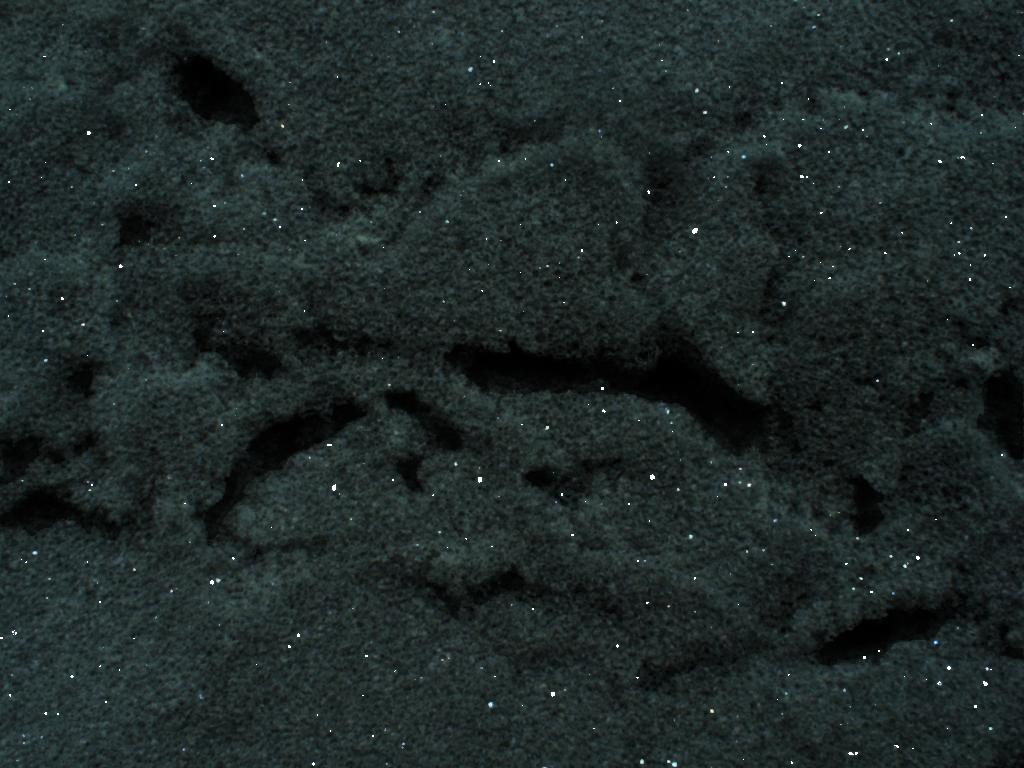
\includegraphics[scale=.12]{image_eps/shadow_classify/thresh=110.eps}
\label{fig:subfig3} } \caption{a) Direct component of an image computed using
bilinear interpolation, b) after multiplying (a) by the shadow mask, and c)
after adding specularity.} \label{fig:subfigureExample}
\end{figure*}

%There are 2 types of interpolation-horizontal and vertical.In horizontal interpolation images at
%two lighting position (at same height) are known and we need to generate or render image at any
%point which lies between image1 and image2(at same height).



\subsection{Shadow Modeling by Interpolation}
Consider a pair of images of a surface captured from the same view point, but by
moving the light source through a short distance. We note that each pixel
(surface point) belong to one of the three categories:
\begin{enumerate}
\item Pixels that are not in shadow in either image.
\item Pixels that are in shadow in both images.
\item Pixels that are in shadow in only one of the images.
%\item Pixels that are in shadow in image 2 but not in image 1.
\end{enumerate}

For the first two types of pixels, the behavior of the pixels remains same as
the lighting direction changes from one image to other. i.e, the pixels that are
in shadow continue to remain in shadow and that illuminated remain illuminated,
provided the distance between the two images being interpolated is small. The
values of these pixels change smoothly.

Modeling this behavior gives good results on all the datasets that we
considered. However, it is possible that this may not hold for high-frequency
textures as small shadows might appear and disappear quickly at a point with
changes in lighting direction. Therefore, a denser the sampling of images will
always provide a better estimate. The luminance values of the first two types of
pixels are directly calculated by linear interpolation between the values of the
corresponding pixels in the given two images. One could also attempt higher
order interpolation techniques, given more images of the same type. In practice,
linear interpolation works well, as the variations are often very limited for
the first two types. Given the luminances, $L_1$ and $L_2$ from the
corresponding pixels of images taken from lighting directions $p_1$ and $p_2$,
the value of the interpolated pixel, $L$, at lighting position $p_0$ is given
by:
\begin{equation}
L=\frac{\omega_2 L_1 + \omega_1 L_2}{\omega_1 + \omega_2},
\end{equation}
where $\omega_i = |D(p_0,p_i)|$; $D(p_a,p_b)$ gives distance between lighting
directions at $p_a$ and $p_b$.

In case of a pixel that transitions from shadow to light (or the reverse), the
transition is quick, though not instantaneous. We model this behavior using a
sigmoid function. As the light source moves from the position of the first
image($p_1$) to  the second($p_2$), there is a point $p_x$ around which the
pixel quickly emerges out of the shadow and then remains illuminated for the
rest of the light motion. The transition would be abrupt except for the
diffraction of light around the edge causing the shadow. Given the illuminations
of the shadow ($L_s$) and non shadow ($L_{ns}$) pixels, and the position $p_x$
at which the transition occurs, the illumination at position $p_0$ can be
approximated by a sigmoid of the form:


\begin{equation}
L = L_{s} + \frac{L_{ns} - L_{s}}{1 + \chi e^{-d}},
\end{equation}
where $d = p_0 - p_x$. The slope of the sigmoid function controls the transient
behavior of pixels from shadow to non-shadow region, controlled by the parameter
$\chi$.



This sigmoid function will exhibit different behavior for different pixels. For
example, the pixels that are at the edge of shadows say in the first image, will
come out of the shadow quickly, whereas the pixels that are at the center of the
shadow will continue to remain in shadow region for a longer time as the light
source is moved from $p_1$ to $p_2$. The parameter $C$ varies slightly depending
on the nature of the surface, but can be treated constant for all practical
purposes, provided the light positions are angular measurements. The only
unknown in carrying out the interpolation is the position $p_x$ at which the
transition occurs. One could estimate it in various ways. A quick approximation
may be obtained by counting the number of pixels around the one under
consideration that are in shadow and not.

The only
unknown in carrying out the interpolation is the position $p_x$ at which the
transition occurs.
Consider a pixel $k$ that is in shadow at light position $p_1$. Let $\chi_s$ be the
fraction of neighboring pixels of $k$ that are in shadow in the first image, and
$\chi_{ns}$ be the fraction of neighboring pixels of $k$ that are not in shadow in
the second image. We compute these fractions by taking masks of increasing sizes
until the $0 < \chi_x < 1$. If $\chi_{ns}$ and $\chi_{s}$ are almost equal, then the
transition, $p_x$ occurs around midway between positions $p_1$ and $p_2$. If
$\chi_{ns} >> \chi_{s}$, then $p_x$ is close to $p_1$, and $\chi_{s} >> \chi_{ns}$ indicates
that $p_x$ is far from $p_1$ and close to $p_2$. We define $p_x$ as: 
%as the linear interpolation of $p_1$ and $p_2$ as follows:
\begin{equation}
p_x = \frac{\chi_{ns} p_1 + \chi_s p_2}{\chi_{ns} + \chi_s}
\end{equation}

The above sigmoidal interpolation can be extended to two dimensions, given an
array of image samples with varying lighting positions, and thus one can compute
the shadow image for any given lighting direction. We refer to this image as the
shadow mask. Figure 3 shows the input images and the interpolated image at two
different lighting positions.


The advantage of interpolation is that the physical structure of the material is
taken into account while interpolating, leading to realistic estimations of
shadows. This is implicitly used while considering the neighborhood information
of a pixel. However approach is both memory and compute intensive as one need to
store input images for interpolation, and the computation of each
pixel of the shadow mask involves searching an increasing neighborhood of
pixels. An alternate method is to decide whether a given pixels falls in shadow
or not, independently as a function of just the lighting position. Fig.\ref{fig:figure3} shows 
the input images and the interpolated image at two different lighting positions.


\subsection{Shadow Modeling by Classification}

In our experiments, we note that most pixels fall under shadow from the effect
of at most two neighboring structures. Hence, a biquadratic classifier boundary
is adequate to decide whether for a given lighting direction, the pixel will be
in shadow or not. The direct component of input images are binarized using
thresholding and used as training data. After the classification, each pixel in
new image is labeled as shadow or non-shadow.

\begin{equation}
 Ya=b
\end{equation}
\begin{equation}
\resizebox{.81\hsize}{!}{$
\underbrace{\left[ {\begin{array}{cccccc}
 {y_1}^{(0)} & {y_1}^{(1)} & \dots\dots & {y_1}^{(5)}\\
{y_2}^{(0)} & {y_2}^{(1)} & \dots\dots & {y_2}^{(5)} \\
 \vdots &  &  & \vdots \\
{y_n}^{(0)} & {y_n}^{(1)} & \dots\dots & {y_n}^{(5)}
 \end{array} } \right]}_{Y}
\underbrace{\left[ {\begin{array}{c}
a_0\\a_1\\ \vdots \\a_5
 \end{array} } \right]}_{a}
=
\underbrace{\left[ {\begin{array}{c}
b_1\\b_2\\ \vdots \\b_n
 \end{array} } \right]}_{b}$}
\end{equation}where
$y_i$=$[{l_u}^2\ \ {l_v}^2\ \ l_ul_v\ \ l_u\ \ l_v\ \ 1]$ and `n' is the total
number of training images.


However, the direct computation of the classifier from the input images often
results in incoherence between neighboring pixels in an image. To improve this,
we first interpolate the input images to obtain the shadow masks at a larger
number of intermediate positions. These values are then used to train the
classifier. The resulting shadow regions estimated by classifier are very close
to original and more accurate than the images that are directly interpolated
from the input images shown below in Figure 4 a-c.

%%%%%%%%%%%%%%%%%FIGURE NO 4 Shadow by classification%%%%%%%%%%%%%%%




Once the classifier is trained, the distance of a point classified as shadow
from the decision boundary can be thought of as the distance from the point of
transition from light to shadow. We use this distance to decide the darkness of
a shadow pixel. The pixel which lies in the region of strong shadows will have a
greater value of absolute distance from the decision boundary than the pixel
which is in a region of diffused shadow or is at the edge of a shadow (See
Figure 5).

%%%%%%%%%%%%%%%%%FIGURE NO 5...Binarised Image of shadow%%%%%%%%%%%%%%%
\begin{figure}[h]
\centering \subfigure[]{

\includegraphics[scale=.15]{image_eps/Binary_Image/cloth/45_orig.eps}
\label{fig:subfig1} } \subfigure[]{

\includegraphics[scale=.15]{image_eps/Binary_Image/cloth/45_hyp.eps}
\label{fig:subfig2} } \subfigure[]{

\includegraphics[scale=.15]{image_eps/Binary_Image/cloth/45_interpol.eps}
\label{fig:subfig3} } \subfigure[]{
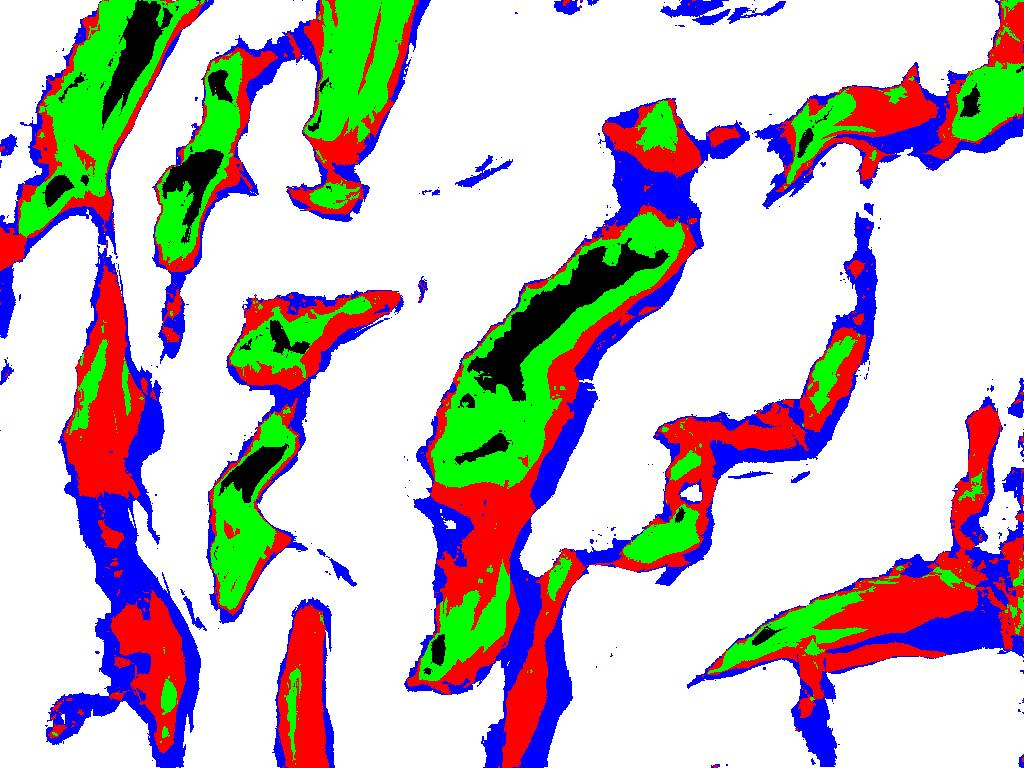
\includegraphics[scale=.15]{image_eps/Binary_Image/cloth/shadow_dist_col.eps}
\label{fig:subfig4} }  \caption{a) Binarized image of cloth shadow, b) binary
image as rendered by classification technique, c) binary image obtained using
interpolation, d) distance image of pixels from classifier boundary. Blue pixels
are closest to the hyperplane and include pixels at the edge of a shadow or
pixels present in the region of diffused shadow. Black color pixels are the
farthest from the hyperplane and represent region of strong and dense shadow.}
\label{fig:subfigureExample}
\end{figure}

We use this binary image to make  a mask where each non-shadow pixel is given a
value of 1 and shadow pixels are given values between 0 to 1 based on their
distance from the hyperplane. The greater the distance, the farther the pixel is
in shadow and thus smaller is the value. Now, since the direct component is
devoid of color variation the change in chrominance value of direct image is
very minimal. Thus using a bilinear function
\begin{equation}
L(l_u,l_v) = \alpha l_u + \beta l_v +\gamma,
\end{equation}
an interpolated image is generated (Figure 4(a)). This image is then multiplied
with shadow mask. Biquadratic function (equation 8) can also be used for
interpolation. Using either of the function for interpolation leads to the
smoothening of shadows. Therefore we multiply this image with a mask described
above to get the shadowed new image (Figure 4b). The value of non-shadow pixels
are not affected but the values of the shadow pixels are attenuated by the
multiplication with the shadow mask. The classification technique thus enables
us to render each pixel independently, increasing the speed of rendering and
making it suitable for processing on the GPUs. The pseudo code for shadow modeling by
classification is given in Algorithm 1.
\begin{algorithm}
\caption{Shadow modeling by classification}
\begin{algorithmic}[1] 
\REQUIRE Binarized direct component training images
%\STATE $y \leftarrow 1$
\STATE Take shadow pixels as negative samples and non-shadow pixels as positive samples.
\STATE Learn the hyper plane (Ya=b) per pixel using pseudo inverse technique.
%\STATE Feature vector: $[{l_u}^2\ \ {l_v}^2\ \ l_ul_v\ \ l_u\ \ l_v\ \ 1]$ where $l_u$ and $l_v$ are given lighting direction in XY plane
\STATE Classify pixels for a given lighting direction
$$
Img(i,j) = \left\{ \begin{array}{rl}
  1 &\mbox{ if $Ya>0$} \\
  0 &\mbox{ otherwise}
       \end{array} \right.
$$
%\IF{$n < 0$}
%\STATE $X \leftarrow 1 / x$
%\STATE $N \leftarrow -n$
%\ELSE
%\STATE $X \leftarrow x$
%\STATE $N \leftarrow n$
%\ENDIF
%\WHILE{$N \neq 0$}
%\IF{$N$ is even}
%\STATE $X \leftarrow X \times X$
%\STATE $N \leftarrow N / 2$
%\ELSE[$N$ is odd]
%\STATE $y \leftarrow y \times X$
%\STATE $N \leftarrow N - 1$
%\ENDIF
%\ENDWHILE
\ENSURE shadow mask image 
\end{algorithmic}
\end{algorithm}


\subsection{Modeling the Specularity}

Specularity is the visible appearance of specular reflections. It determines the
brightness and location of the specular highlights, given a lighting direction.
In case of PTMs, the ability to model the specularity is sacrificed due to fixed
viewing direction. PTMs use a biquadratic interpolation model due to which the
intermittent highlights, inherently present in many texture surfaces, are
completely washed out.

We model the specular highlights separately from the base reflection and
shadowing in the direct component. The value of pixels showing these highlights
fall off very sharply as lighting direction is changed. One could use any sharp
falling function such as a Gaussian with very small variance or an exponential
to model it. We model the specular highlights, S, as:

\begin{equation}
S= \eta exp-\left[\frac{({l_u-\mu_x})^2 + ({l_v-\mu_y})^2}{\delta}\right],
\end{equation}
where $\mu_x$ and $\mu_y$ are the lighting direction coordinates at which
specularity is maximum, $l_u$ and $l_v$ are the current lighting directions.
$\eta$ and $\delta$ are the parameters that control the
magnitude and fall-off of this function. The highlights also can have a tint
based on the nature of reflection. In this case, one can multiply the above
%We multiply above
function with a single chrominance value to achieve realistic estimation.

We note that the modeling of highlights is tricky as one can observe highlights
only if one of the original images contain it. Hence the highlights estimated
are often inaccurate, although realistic (see Figures 9d,e). Figure 4(c) shows
the final image after multiplying the bilinearly interpolated image with shadow
mask and adding specularity.

%%%%%%%%%%%%%%%%%FIGURE NO 6_ global component of cloth%%%%%%%%%%%%%%%
\begin{figure}[t]
\centering \subfigure[]{
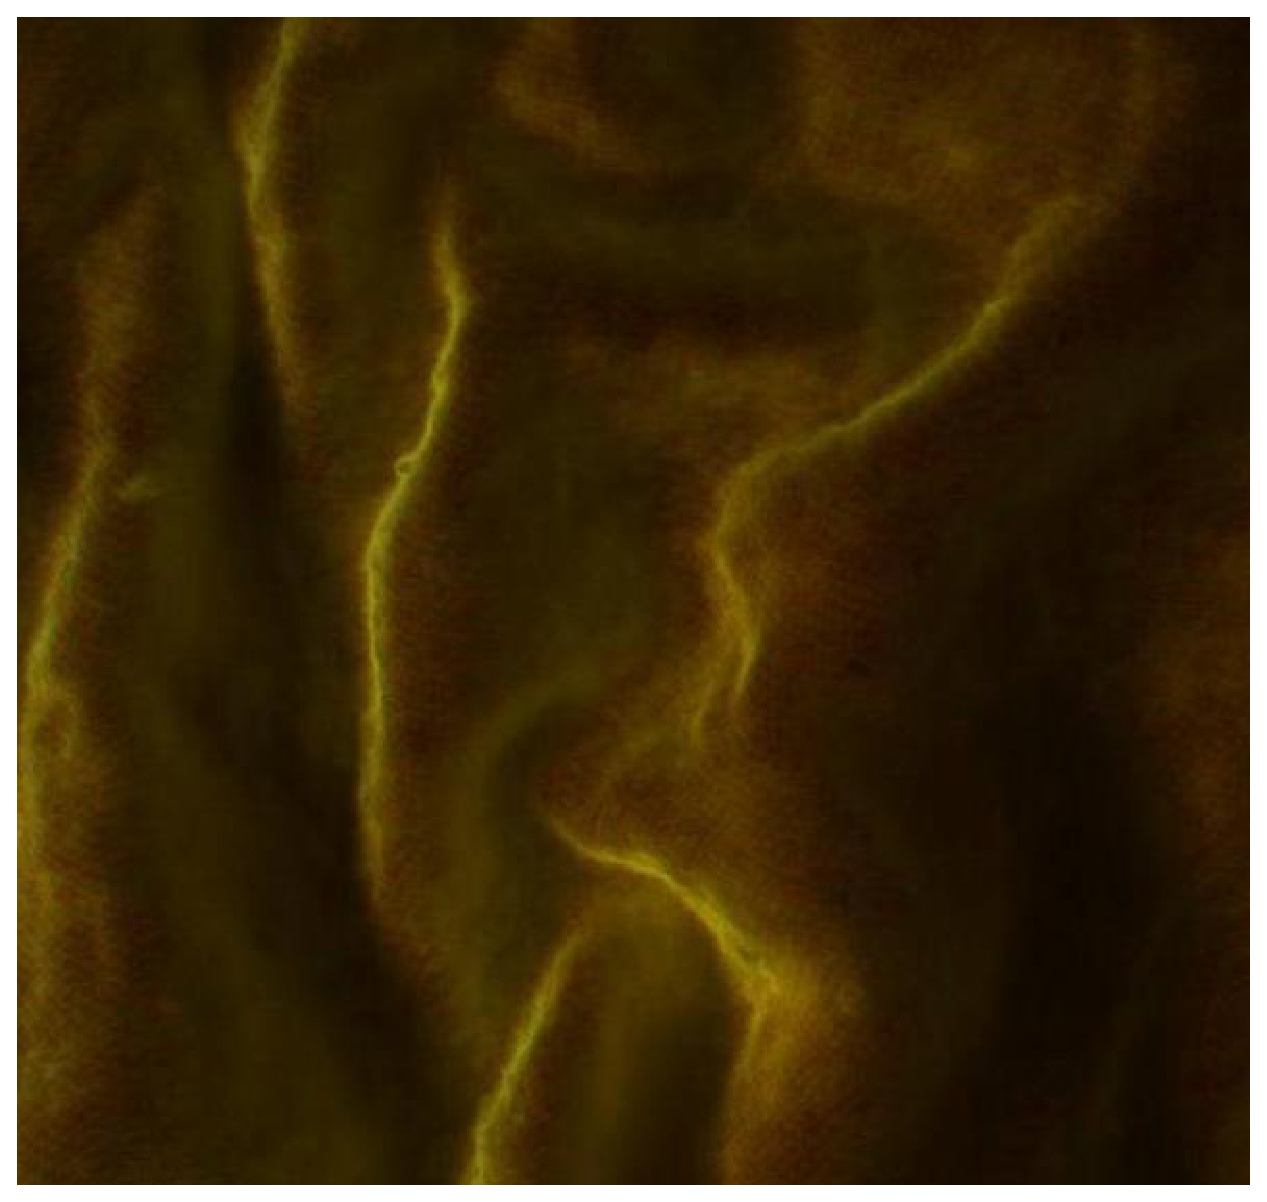
\includegraphics[scale=.15]{image_eps/global/cloth/crop_theta=30_phi=105_Orig.eps}
\label{fig:subfig1} } \subfigure[]{
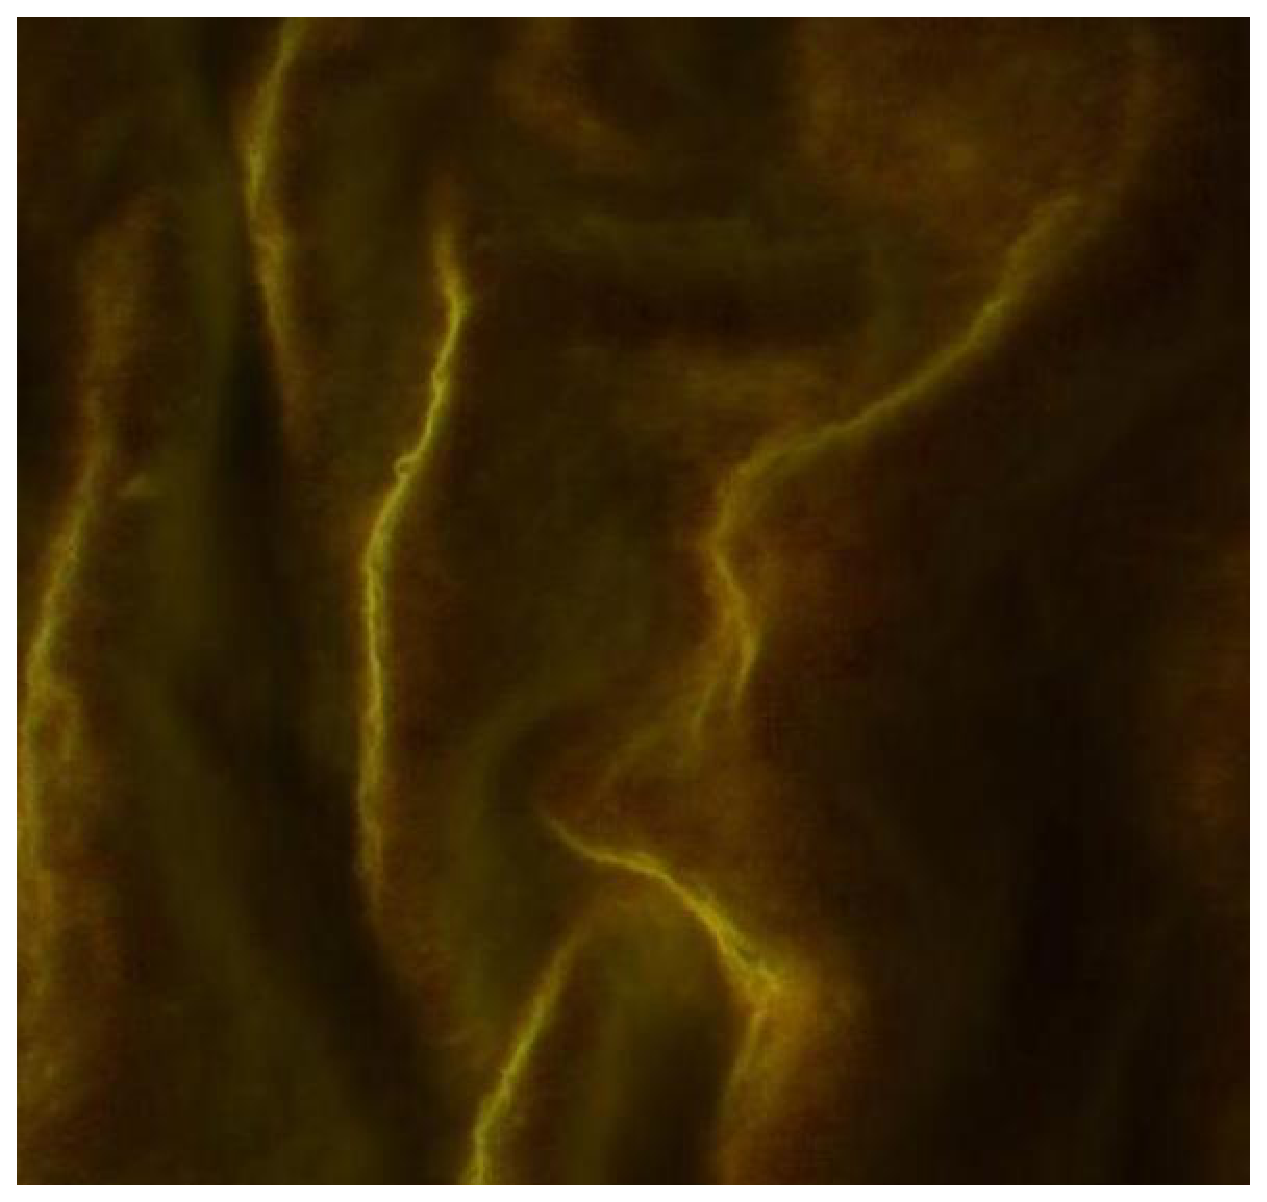
\includegraphics[scale=.15]{image_eps/global/cloth/crop_theta=30_phi=105_gauss.eps}
\label{fig:subfig2} } \subfigure[]{
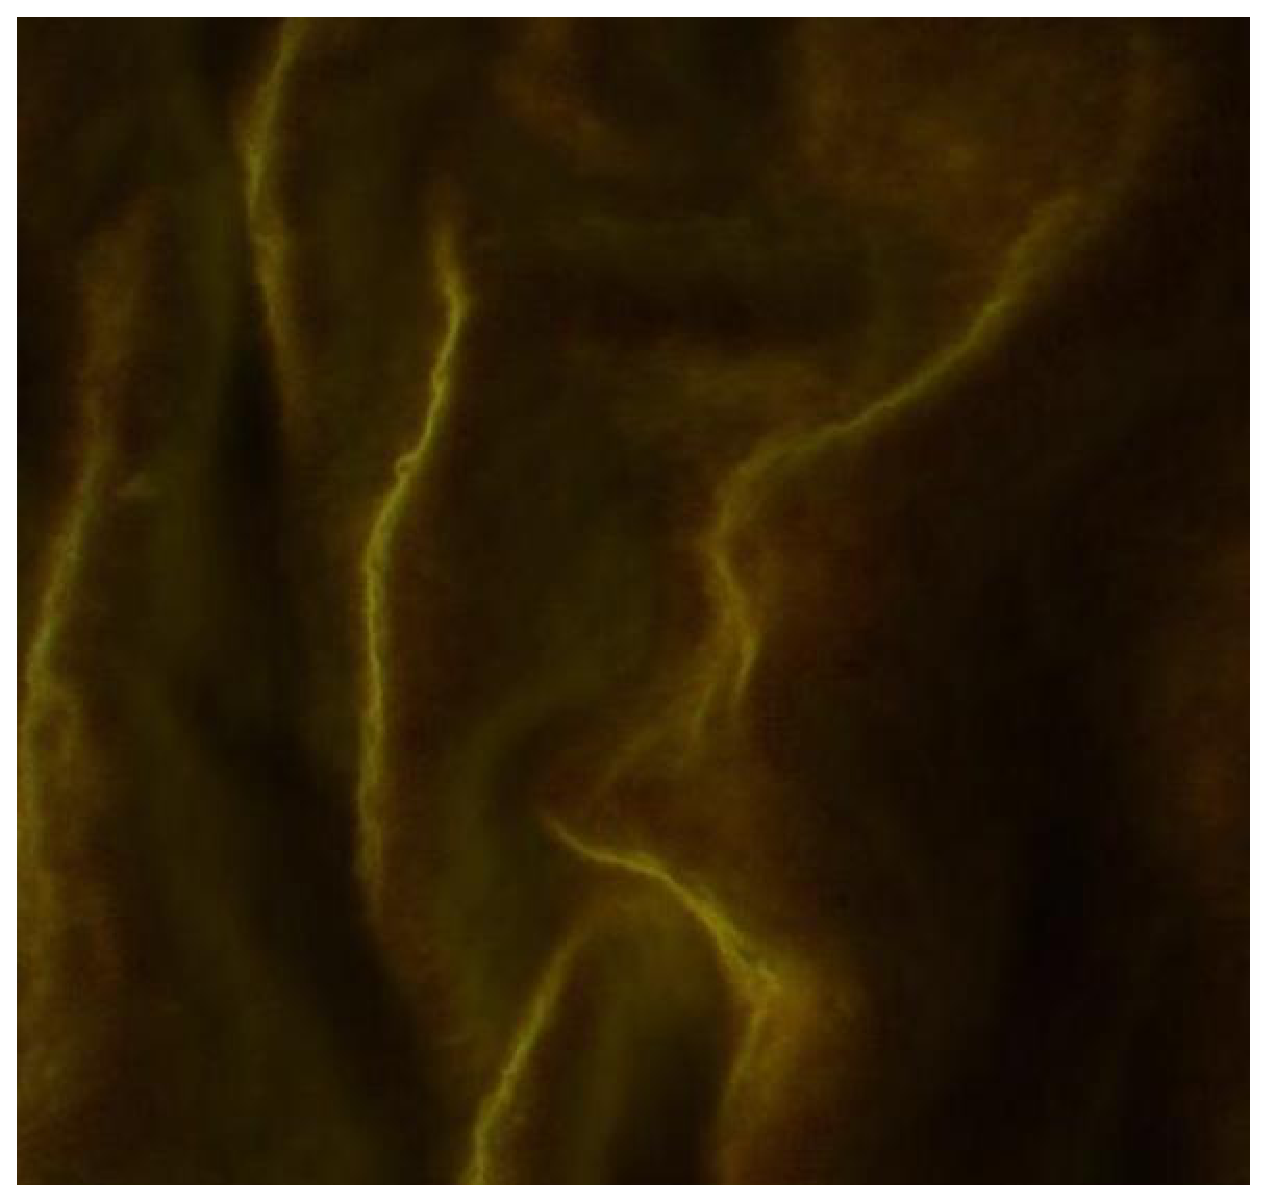
\includegraphics[scale=.15]{image_eps/global/cloth/crop_theta=30_phi=105_PTM.eps}
\label{fig:subfig3} } \subfigure[]{
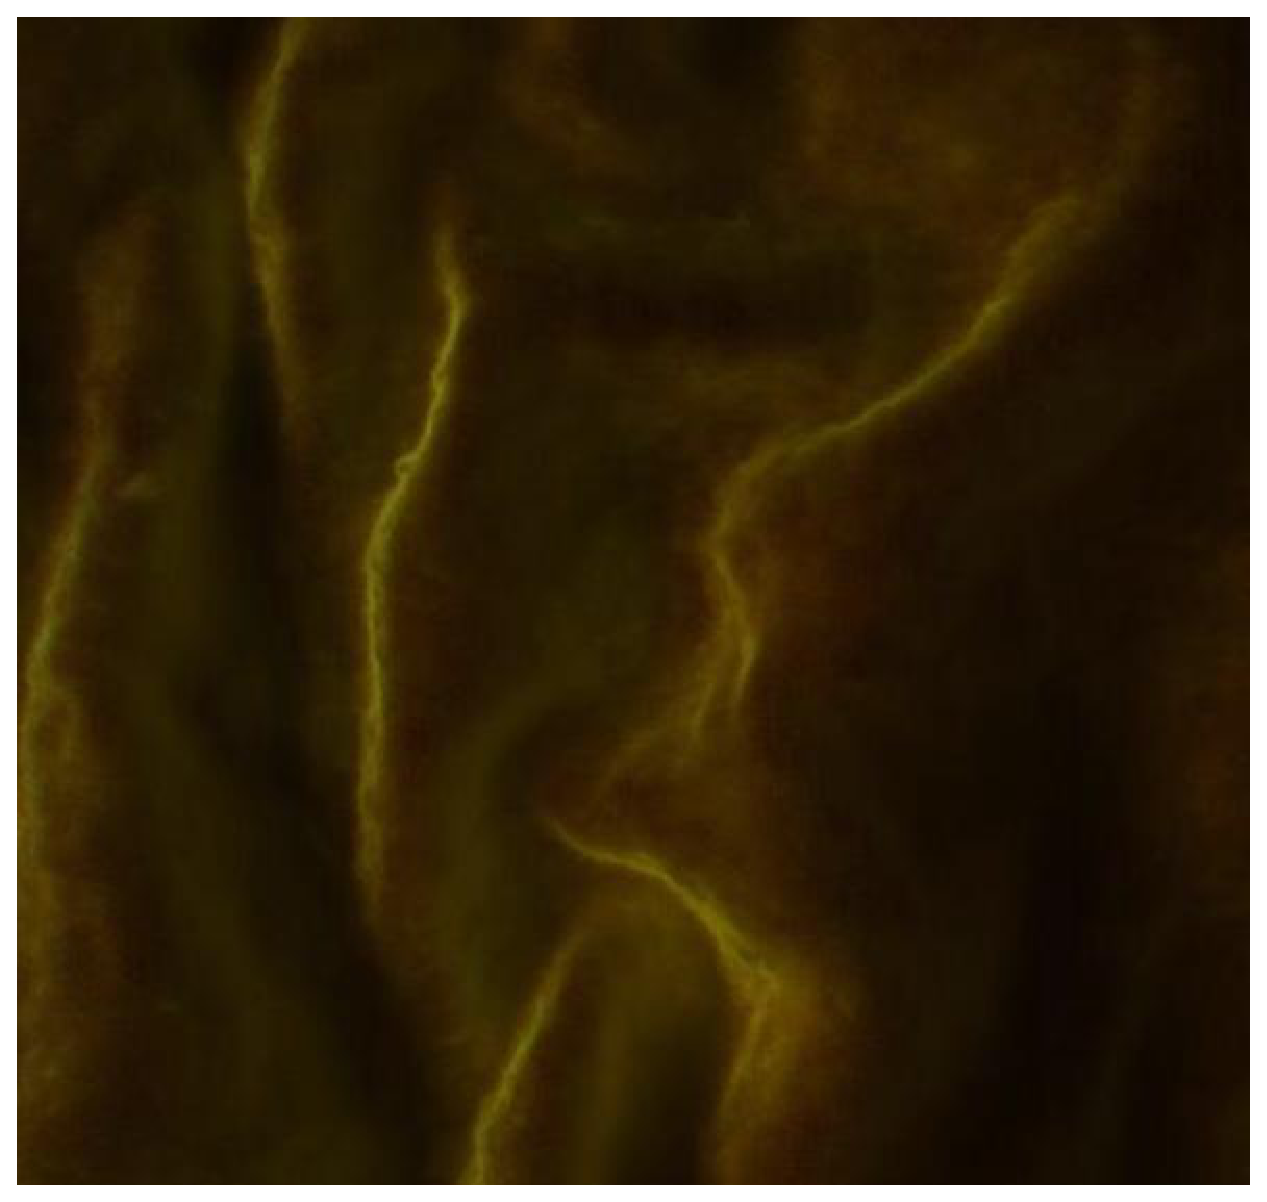
\includegraphics[scale=.15]{image_eps/global/cloth/crop_theta=30_phi=105_parabola.eps}
\label{fig:subfig4} } \caption[Optional caption for list of figures] {(a)
Original Global Image (b)Global Image modeled by Gaussian function (c)Global
Image modeled by biquadratic (d)Global image modeled by Parabola.}
\label{fig:globalCloth}
\end{figure}


\section{Modeling Global Component}

The global component of the image is characterized by subsurface scattering,
secondary illumination, diffuse inter-reflections, volumetric scattering and
translucency. These are not sharply varying phenomena and therefore the
variation of luminance can be modeled using appropriate function. However, the
inherent interaction between different parts of the surface in global
illumination means that the chrominance of a point can change with change in
lighting direction. The global part of the image is responsible for the feeling
of depth and life in many surfaces. As we separate the modeling of global
component, the color values of the image rendered are closer in value to the
original image and better than the images generated by PTM. From our experiments
on various surfaces, the global component of illumination tends to be maximal
when the illumination is perpendicular to the surface, and drops off in a
symmetric fashion. We experiment with the following function for modeling the
global component: a)Gaussian b)biquadratic polynomial, and c)paraboloid.


In Gaussian function we model the luminance as a gaussian function of lighting
direction:
\begin{equation}
L(l_u,l_v)=K\exp-(al_u^2 + bl_v^2 + cl_ul_v + dl_u + el_v +f  ).
\end{equation}

The equation may be rewritten as:
\begin{equation}
al_u^2 + bl_v^2 + cl_ul_v + dl_u + el_v -k= -\ln(L(l_u,l_v)),
\end{equation}
resulting in the following system of linear equations for parameter estimation:

\begin{center}
$\left[ {\begin{array}{cccccc}
 l_{u1}^2 & l_{v1}^2 & l_{u1}l_{v1} & l_{u1} & l_{v1} & -1 \\
  \dots & \dots  & \dots & \dots & \dots &  \dots \\
\dots & \dots  & \dots & \dots & \dots &  \dots \\
\dots & \dots  & \dots & \dots & \dots &  \dots \\
\dots & \dots  & \dots & \dots & \dots &  \dots \\
l_{un}^2 & l_{vn}^2 & l_{un}l_{vn} & l_{un} & l_{vn} & -1
 \end{array} } \right]
$
$\left[ {\begin{array}{c}
a\\b\\c\\d\\e\\k
 \end{array} } \right]
$=
$\left[ {\begin{array}{c}
-\ln(L_1)\\ \dots\\ \dots\\ \dots \\ \dots \\ -\ln(L_n)
 \end{array} } \right]
$\newline
\end{center}

The above system of equations can be solved using SVD and the coefficients
$a,b,c,d,e,$ and $k$, can be estimated per pixel. Biquadratic polynomial, also
used in modeling PTMs \cite{B6}, can be a good choice here because of the
absence of sharply varying features. The function is given by:
\begin{equation}
L(l_u,l_v) = al_u^2 + bl_v^2 + cl_ul_v + dl_u + el_v +f
\end{equation}

The paraboloid may not be as accurate as above functions and can lead to some
smoothening but they are computationally efficient with 5 coefficients per pixel
\begin{equation}
L(l_u,l_v)= al_u^2 + bl_v^2  + cl_u + dl_v +e
\end{equation}

Figure[6 a-d]\footnote{Please view these images in soft copy for better clarity}
shows the global component as modeled by each of the above functions. We see
that the gaussian model provides the most accurate estimation of global
component although all three models are similar in performance to visual
inspection. One could hence use the paraboloid for purposes of efficiency and
storage.

%%%%%%%%%%%%%%%%%FIGURE NO 7....graph plots  %%%%%%%%%%%%%%%
\begin{figure}[t]
\centering
\subfigure[]{
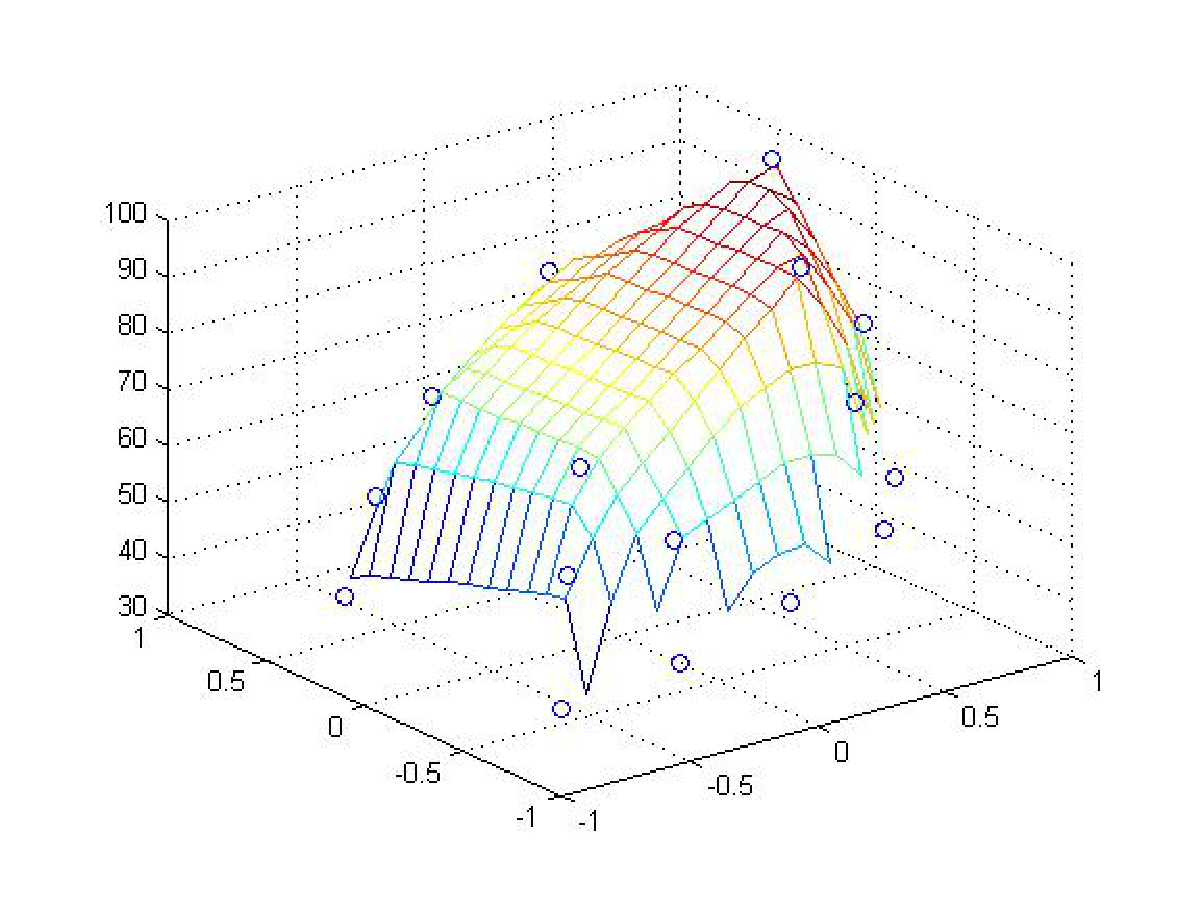
\includegraphics[scale=.3]{image_eps/global/cloth/574_236_orig.eps}
\label{fig:subfig1}
}
\subfigure[]{
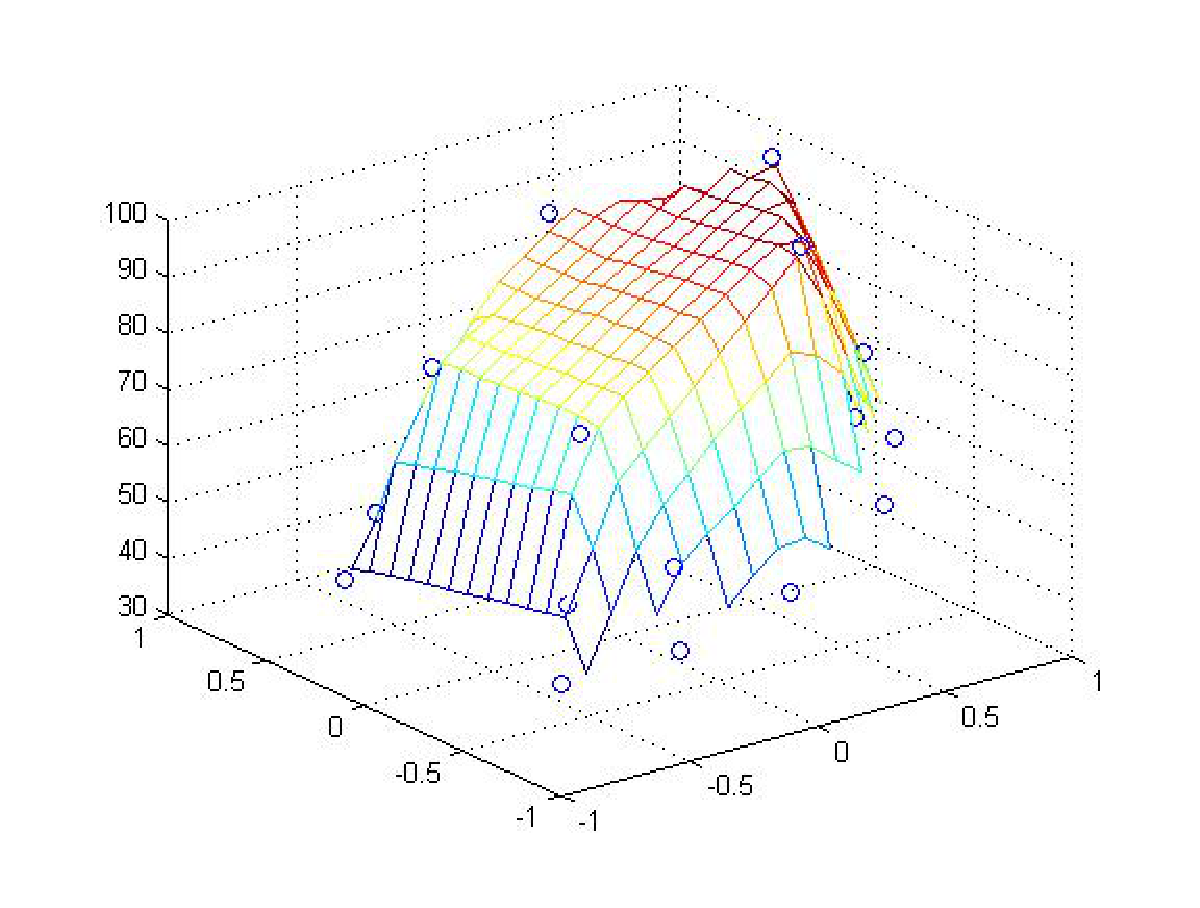
\includegraphics[scale=.3]{image_eps/global/cloth/574_236_gauss.eps}
\label{fig:subfig2}
}
\subfigure[]{
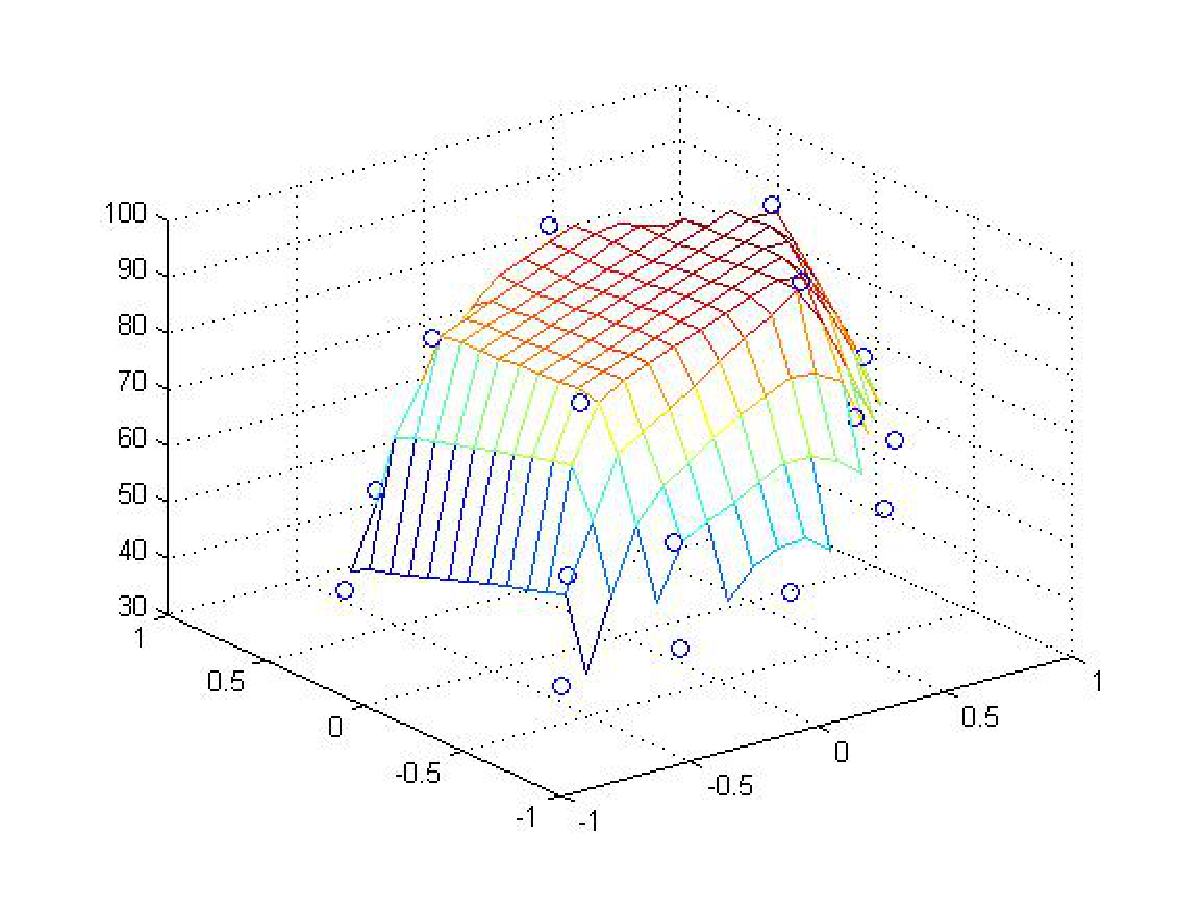
\includegraphics[scale=.3]{image_eps/global/cloth/574_236_PTM.eps}
\label{fig:subfig3}
}
\subfigure[]{
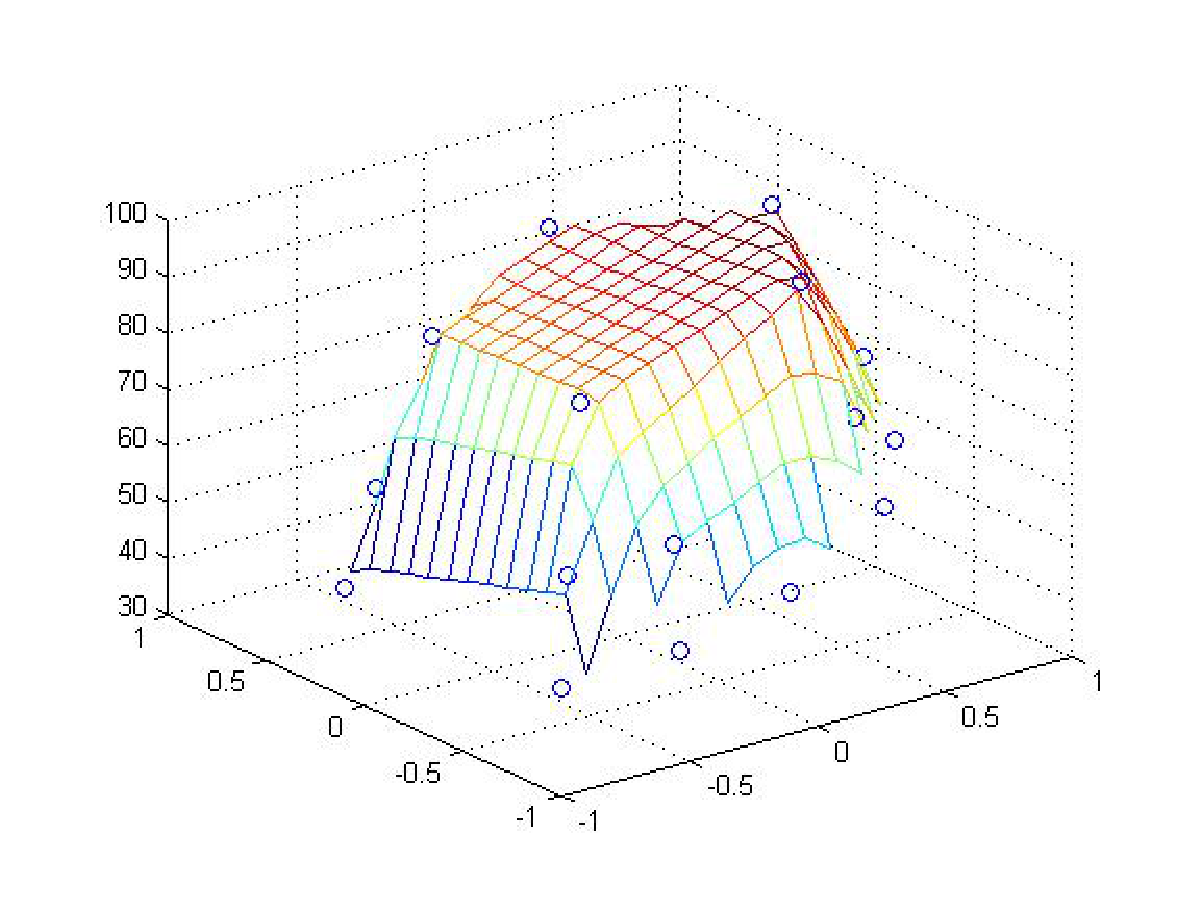
\includegraphics[scale=.3]{image_eps/global/cloth/574_236_parabola.eps}
\label{fig:subfig4} }
\caption{Comparison of luminance
 at a pixel as modeled by different functions: a) original
function plot at that pixel b)By Gaussian c)By Biquadratic
d)By Parabola.}  \label{fig:subfigureExample}
\end{figure}


The graphs shown in Figure[7a] shows how the luminance of a given pixel varies
with different lighting directions. Figure [7 (b)-(d)] shows the luminance of
this pixel as a function of lighting direction when modeled using the different
functions mentioned above. It is clear from the plots that gaussian is more
accurate than the other two functions especially at the peak value. The mean
squared error over a sampled set of points from different surfaces is shown for
comparison in table 1. Experimentally and visually, the Gaussian model best fits
the observations.

%\begin{center}
\begin{table}[ht]
\centering
 \caption{Root Mean Square Error Comparison}
  \begin{tabular}{| l | c | c | c |}
    \hline
    Dataset & Gaussian & Biquadratic & Parabolic\\ \hline
    Sponge & 2.70 & 3.64 & 3.26\\ \hline
    Cloth &  3.60 & 6.01 & 4.41\\ \hline
    Granite & 2.81 & 3.99 & 3.25\\ \hline
    Sand & 2.66 & 4.09 & 3.97\\ \hline
  \end{tabular}
\end{table}

\section{Data Acquisition}
%\label{sec:2}

The setup required to capture input images include projector and a camera. The
camera is mounted vertically above a table that holds the surface (See Figure \ref{fig:17}). The scene is
illuminated using a high frequency checkerboard pattern using the projector. The
projector is moved to different lighting positions for the purpose of obtaining
images with different lighting directions. The distance of the projector from
the scene remains fixed, and only its height and position is changed. This
enables us to capture images with lighting from a hemispherical set of world
coordinates. We capture 30 images from different lighting directions. For each
lighting direction, using component separation technique described in \cite{B4},
25 images are captured and then we separate the image into its global and direct components. The resultant
dataset used for modelling contains 60 images per surface, with 2 from each lighting direction.

We collect multiple images of a static object with a static camera under varying
lighting conditions. The
camera is mounted vertically above a table that holds the surface. Since the camera is fixed, we avoid the
need for any camera caliberation. 
The scene is illuminated using a high frequency checkerboard pattern with the help of the projector. The
projector (light source) is moved to different lighting positions for the purpose of obtaining
images with different lighting directions. 
The distance of the projector from
the scene remains fixed, and only its height and position is changed. This
enables us to capture multiple images with varying light source direction from a hemispherical set of world
coordinates. We capture images from 30 different lighting directions and for each
lighting direction, using component separation technique described in \cite{A9},
we separate the image into its global and direct components. We capture 5-6 additional images which are used as 
benchmark images for comparing results.  

\section{Experimental Results and Analysis}

The component based modeling proposed in this paper has been applied on various
natural material textures. We present qualitative and quantitative assessment on
texture images as obtained from our method and that obtained from the PTM over
different natural material surfaces. Figure 9(a)-(l) \footnote{View images in
soft copy for better clarity} shows qualitative results where we compare the
ground truth images with images obtained from our technique and with PTMs. The
texture of sand when modeled using CBM technique, preserves prominent shadow
regions where as these regions are significantly washed out in PTM images(Figure
9(a)-(c)) The sponge texture (Fig 9(d)-(f)) shows a very noticeable difference
between the two techniques \footnote{Please refer the supplementary video for a
better comparison between CBM and PTM}.

In the PTM image, there are no sharp shadows, the specularities are washed out
and surface relief is smoothened to some extent whereas in CBM, structural
details are preserved making it look more photorealistic. In Figure 9(g)-(l),
two different granite surfaces are modeled. Once again PTM smoothens sharp
shadows, while they are preserved in the CBM rendered images.

For quantitative comparison, we capture additional images from known lighting
directions during the capture phase. Generic measures such as PSNR only gives
the average differences, and are not visually significant. We compute the
absolute differences between each pixel values and analyze the distribution of
these values. The differences between the original image and the image rendered
using CBM and PTM are also plotted as a boxplot (see Figure 8).


%%%%%%%%%%%%%%%%FIGURE NO 8%%%%%%%%%%%%%%%%
\begin{figure}[h!p]
\centering
\subfigure[]{
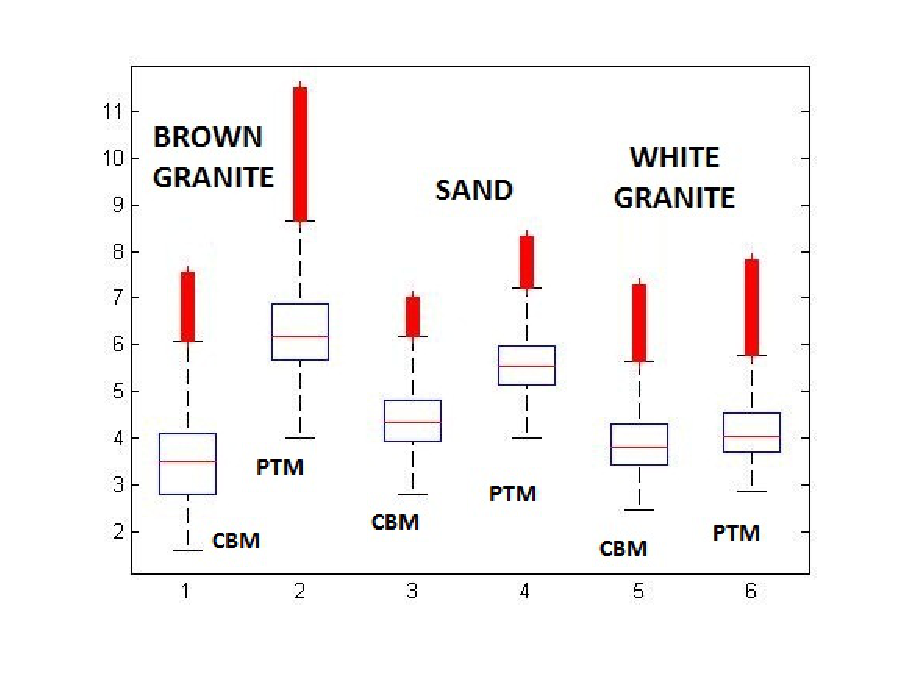
\includegraphics[scale=.42]{image_eps/boxplot/plot1.eps}
\label{fig:subfig1}
}
\subfigure[]{
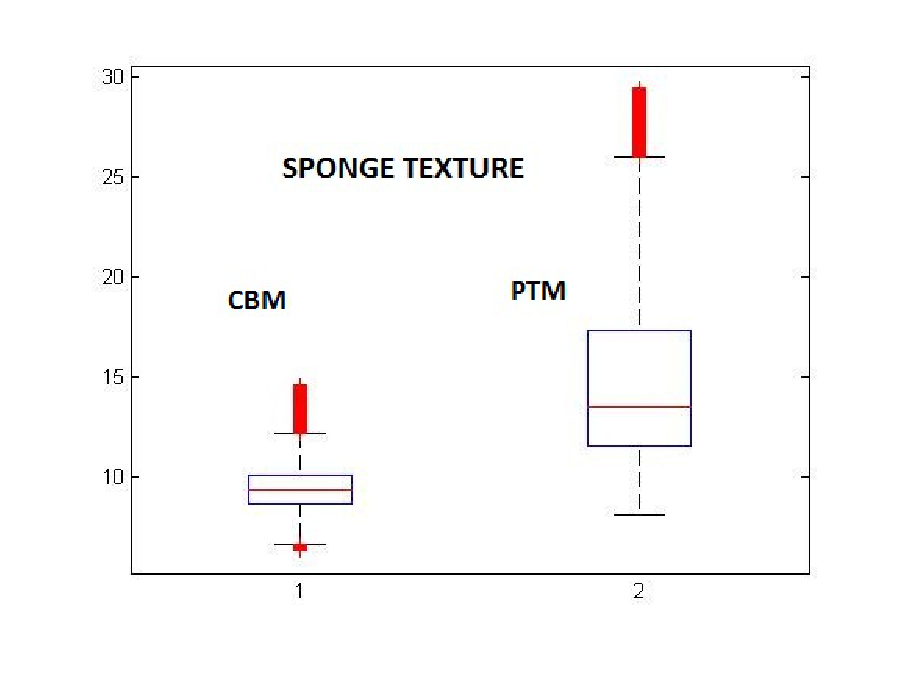
\includegraphics[scale=.42]{image_eps/boxplot/sponge2.eps}
\label{fig:subfig2}
}
\caption{Error comparison between CBM and PTM over
different surface textures. Red bars indicate outliers. The red line in the box
is the mean and the blue lines are the 25th and 75th percentile.}
\end{figure}

%%%%%%%%%%%%%%%%%FIGURE NO 9%%%%%%%%%%%%%%%
\begin{figure*}[t]
\centering
\subfigure[Original Sand Texture]{
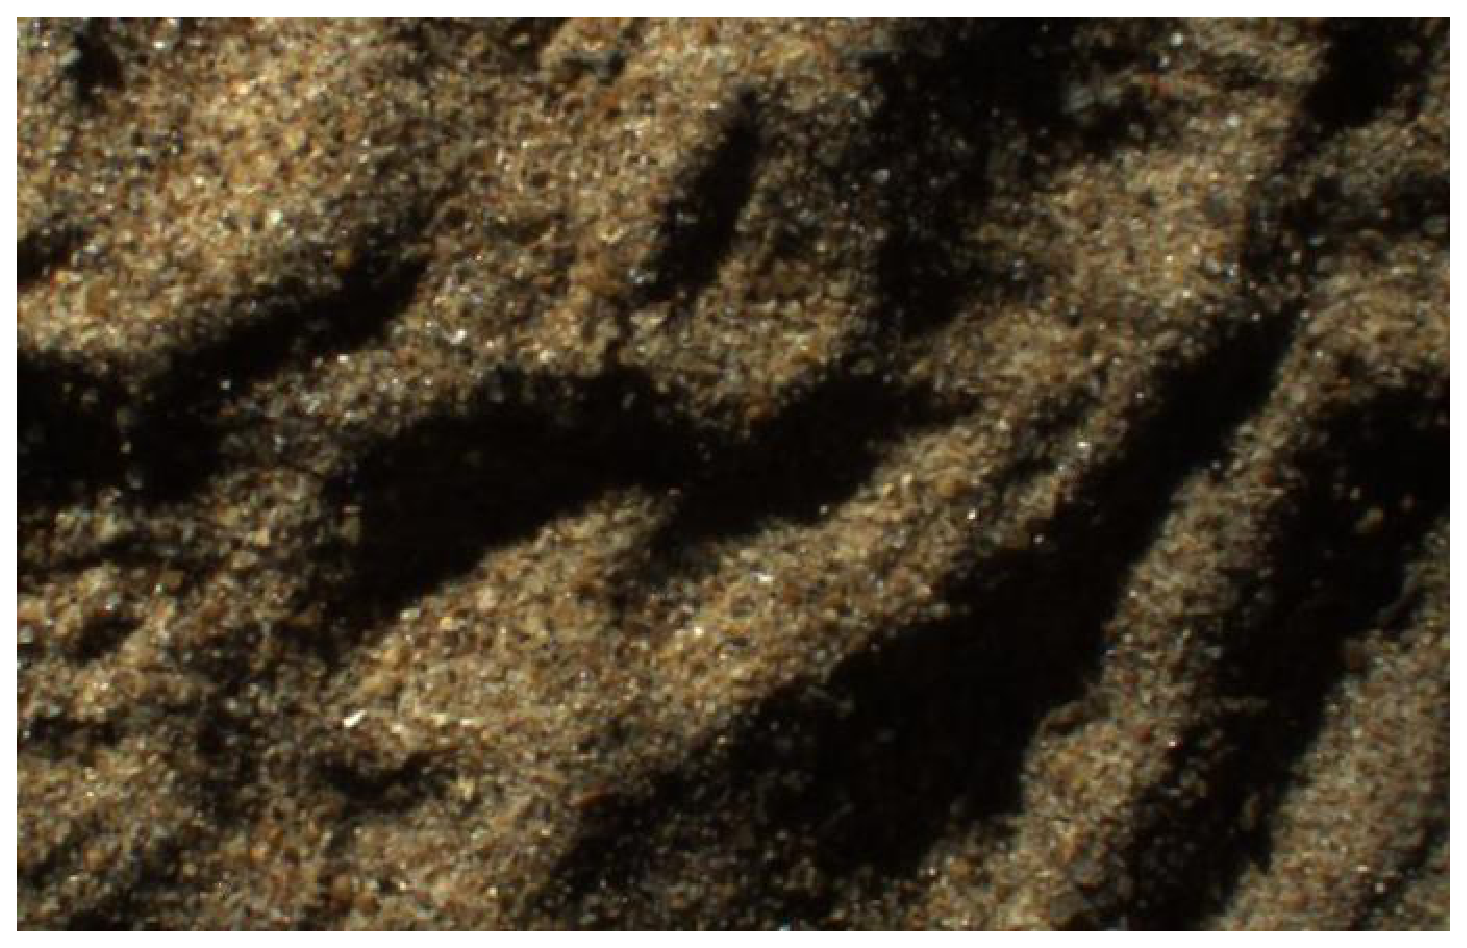
\includegraphics[scale=.205]{image_eps/Data_image/sand/crop_30_orig.eps}
\label{fig:subfig1}
}
\subfigure[Modelled using CBM]{

\includegraphics[scale=.205]{image_eps/Data_image/sand/crop_30_inter2.eps}
\label{fig:subfig2}
}
\subfigure[Modelled using PTM]{
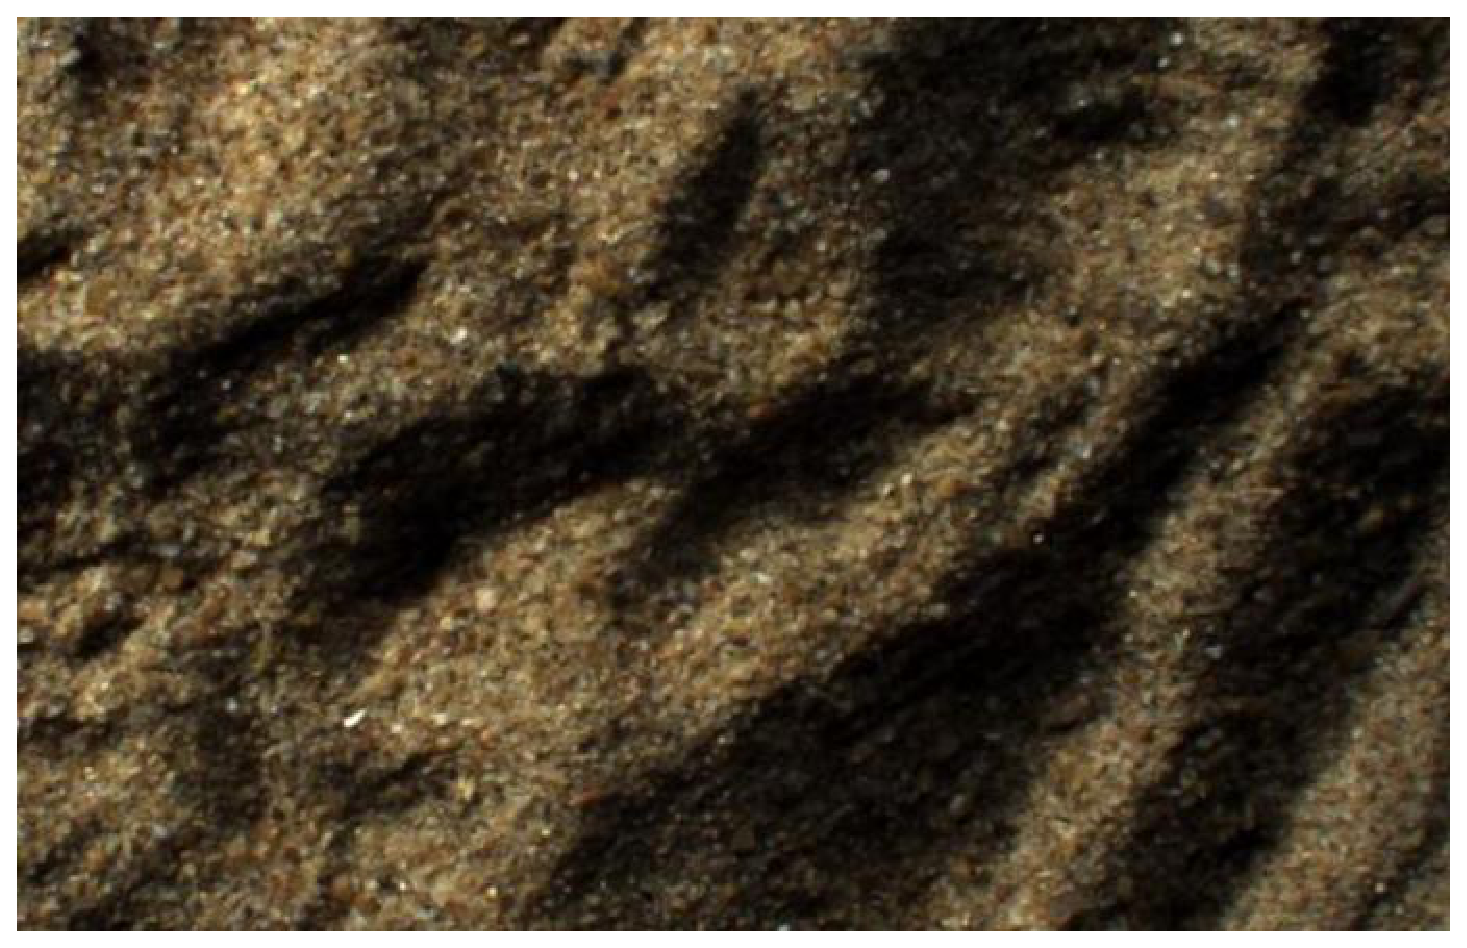
\includegraphics[scale=.205]{image_eps/Data_image/sand/crop_30_PTM.eps}
\label{fig:subfig3}
}

\end{figure*}

\begin{figure*}[ht]
\centering
\subfigure[Original Sponge Texture]{

\includegraphics[scale=.135]{image_eps/4.eps}
\label{fig:subfig1}
}
\subfigure[Modelled using CBM]{

\includegraphics[scale=.135]{image_eps/5.eps}
\label{fig:subfig2}
}
\subfigure[Modelled using PTM]{

\includegraphics[scale=.135]{image_eps/6.eps}
\label{fig:subfig3}
}
\end{figure*}

\begin{figure*}[ht]
\centering
\subfigure[Brown Granite]{
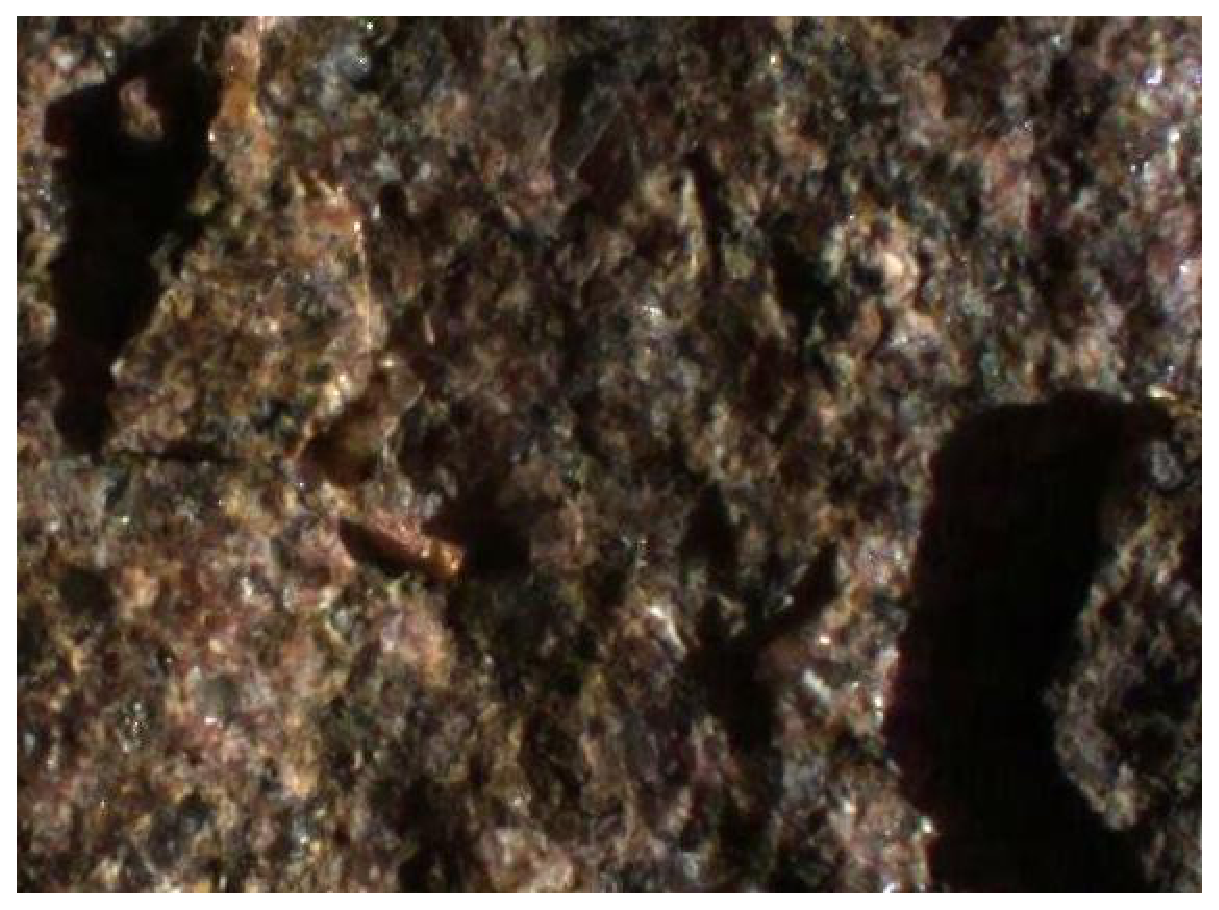
\includegraphics[scale=.24]{image_eps/Data_image/granite2/crop_270_orig.eps}
\label{fig:subfig1}
}
\subfigure[Modelled using CBM]{
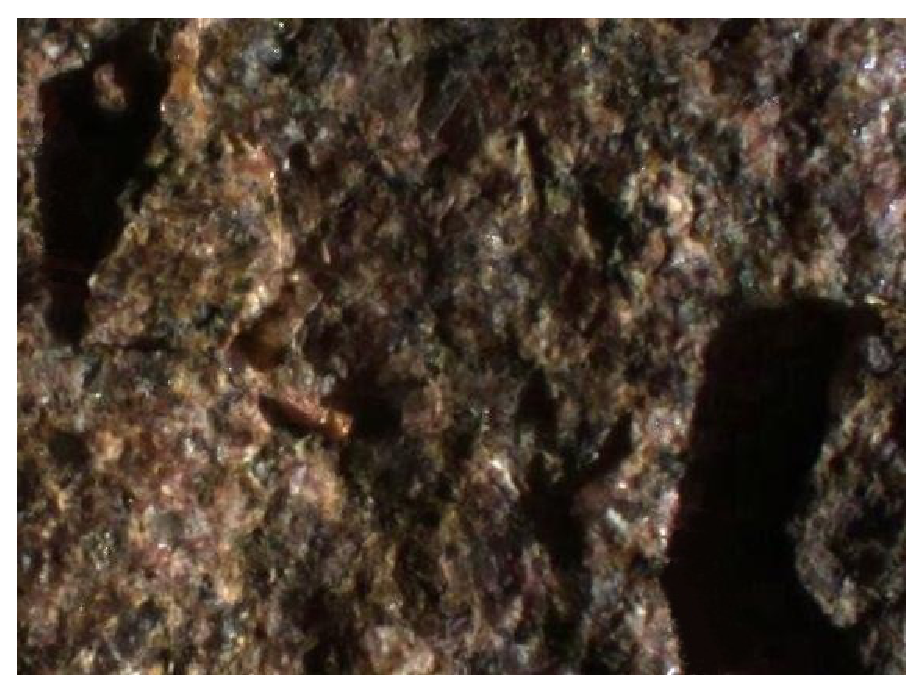
\includegraphics[scale=.32]{image_eps/Data_image/granite2/crop_270_inter_new.eps}
\label{fig:subfig2}
}
\subfigure[Modelled using PTM]{
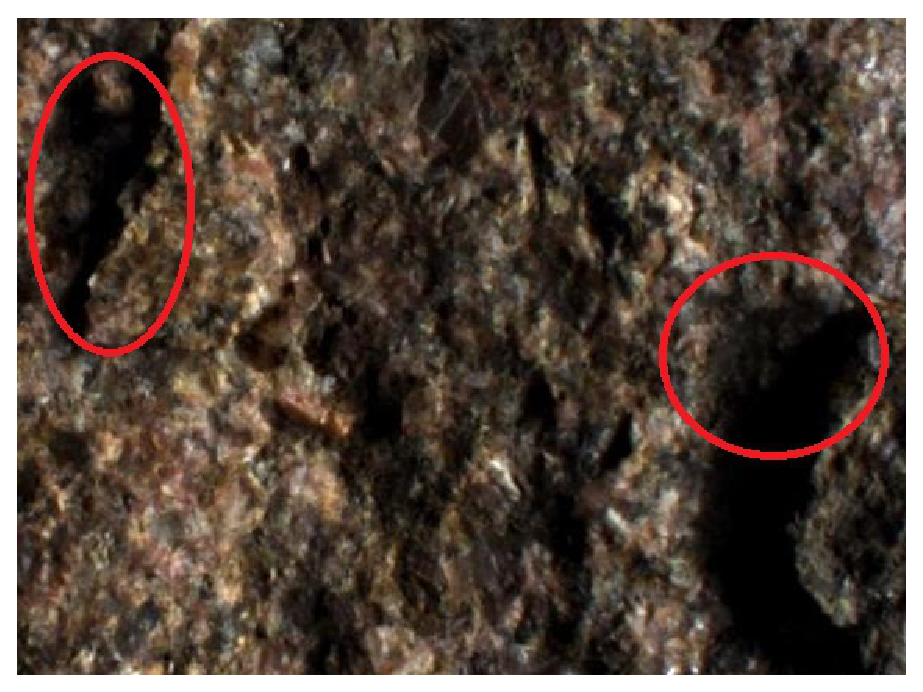
\includegraphics[scale=.32]{image_eps/Data_image/granite2/crop_270_PTM2.eps}
\label{fig:subfig3}
}
%\end{figure*}

\subfigure[Original Cloth Texture]{
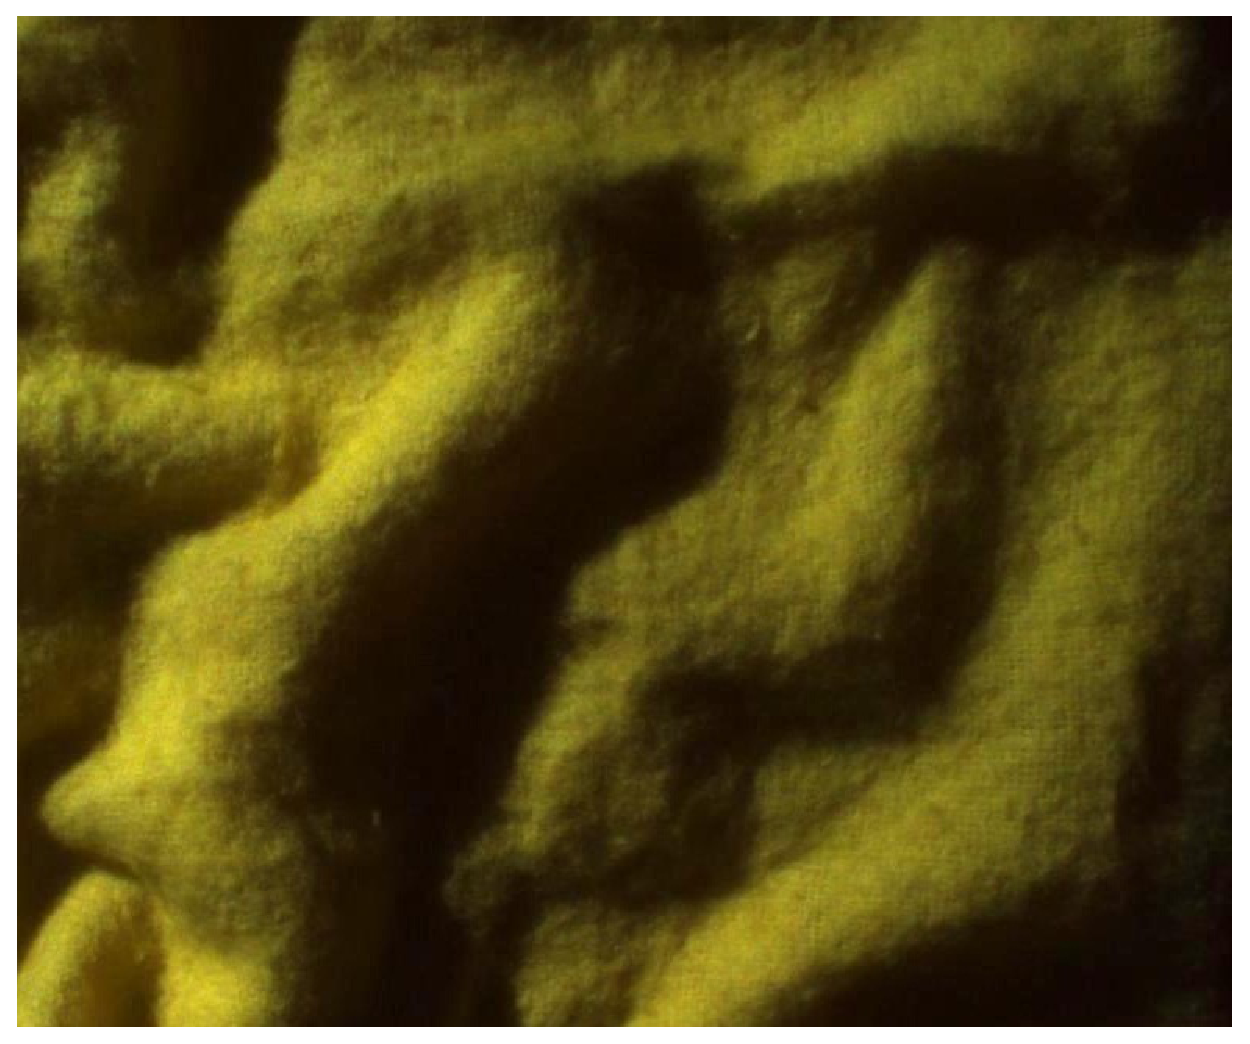
\includegraphics[height=1.25in,width=1.95in]{image_eps/Data_image/cloth_eps/1_45_orig.eps}
\label{fig:subfig1}
}
\subfigure[Modeled using CBM]{
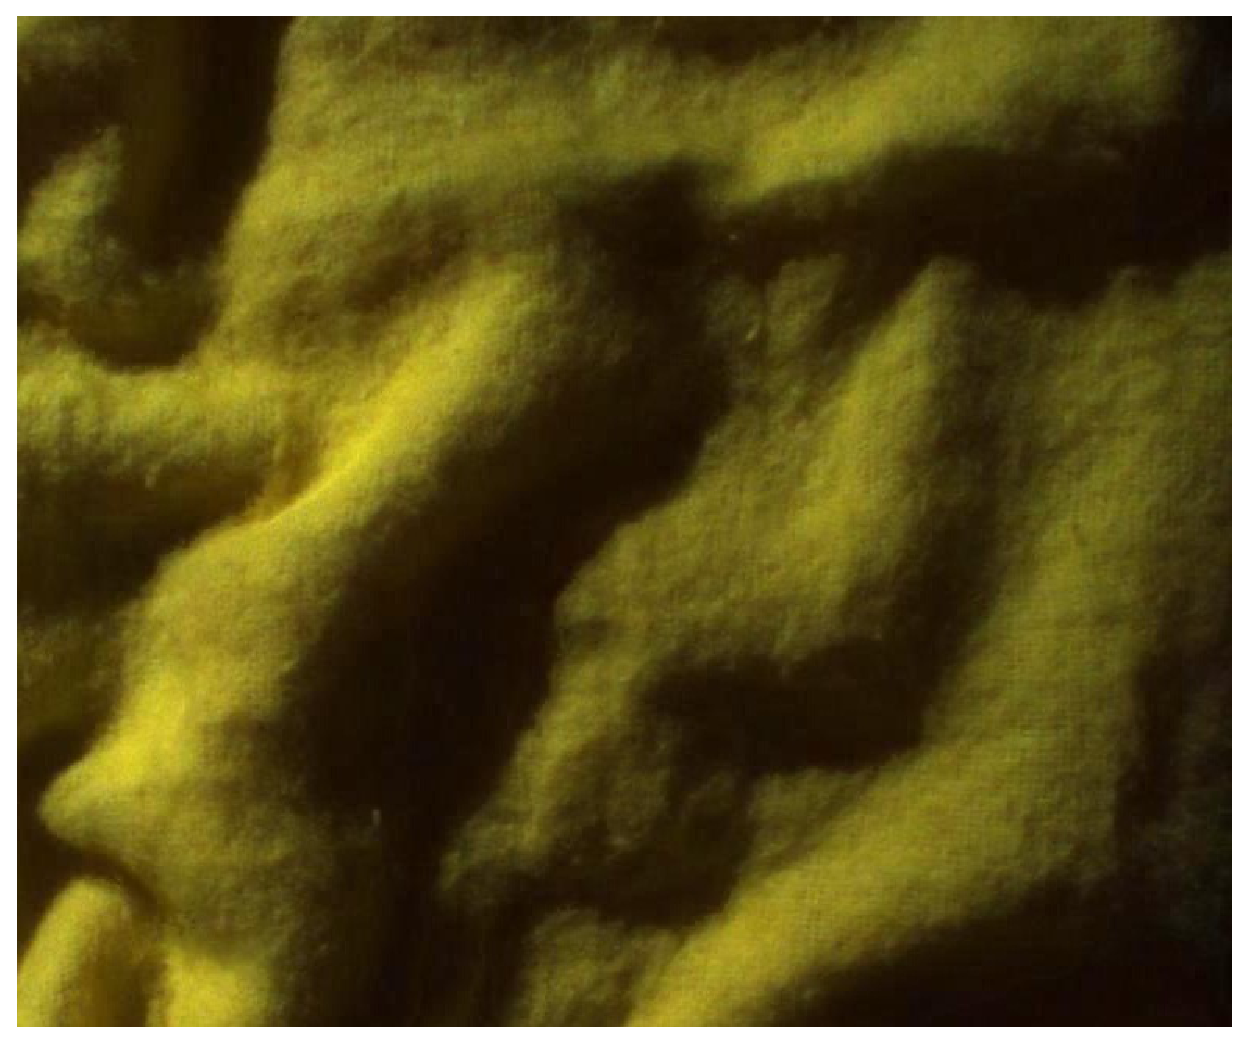
\includegraphics[height=1.25in,width=1.95in]{image_eps/Data_image/cloth_eps/1_45_our.eps}
\label{fig:subfig2}
}
\subfigure[Modeled using PTM]{
\includegraphics[height=1.25in,width=1.95in]{image_eps/Data_image/cloth_eps/1_45_PTM.eps}
\label{fig:subfig3}
}



%\begin{figure*}[ht]
%\centering
\subfigure[Zoomed part of White Granite]{
\includegraphics[scale=.205]{image_eps/Data_image/granite1/crop_286_orig.eps}
\label{fig:subfig1}
}
\subfigure[Modelled using CBM]{
\includegraphics[scale=.205]{image_eps/Data_image/granite1/crop_286_inter.eps}
\label{fig:subfig2}
}
\subfigure[Modelled using PTM]{
\includegraphics[scale=.205]{image_eps/Data_image/granite1/crop_286_PTM.eps}
\label{fig:subfig3}
}

\caption{Comparison of rendering results from Component Based Modeling and PTM
techniques. CBM images have sharp shadows and specularity and also preserve the
appearance of surface relief.}
\end{figure*}

It is clear from the the figure that the average per pixel error and the number
of outlier points are less in the image rendered using component based modeling
technique as compared to those rendered using PTM. However, one should note that
the PTM based models miss the specularities completely, while CBM is possibly
rendering some of the specularities at incorrect positions. This would result in
a higher quantitative error for CBM, while the visual appearance is improved.

In case of brown granite texture (Fig 8a-1,2), one can observe that the number
of outliers are quite high in case of PTM. This is because the texture has
specularities which PTM fails to captures and also the sharpness of edges in
shadow regions are lost. The root mean square error in case of CBM is 3.5 whereas in case of PTM its 6.2. 
If outliers are included then rms becomes 4.9 for CBM and shoots upto 10.1 for PTM.
In case of white granite (Fig 8a-5,6), there is not
much difference in the average errors of the two techniques. For CBM rms error is 3.8 and 4.2 for PTM. As the texture does
not have specularity, also there is not much structural variation and the shadow
regions are small, therefore PTM is able to model it quite well with lesser
errors. However, if we consider sponge texture, the PTM performs quite badly
with average error of around 14 and 75th percentile at 17 whereas average error
of CBM is around 8 with 75th percentile at 10(Figure 8(b)). Sponge is a highly
textured surface with specularities and prominent shadow regions and therefore
PTM produces very bad results as it tends to smoothen out the surface relief.
But component based modeling accurately captures all structural details and thus
rendered image is closer to the original.
Modeling the shadows and specularity separately in CBM also allows us to make rendered images with
multiple light sources, more realistic. Consider Figure 10,
%\footnote{View figure by zooming the page for better clarity and differentiating the images} 
where the sponge texture
is illuminated at 10$^{\circ}$ (from the top of the image), and 180$^{\circ}$
(bottom). Areas that are in shadows for both lighting directions are preserved
as shadow in the resultant image and the specularities have added up. However, with PTM based rendering, shadows tend
to become more washed out with multiple light sources and rendered image is void of specularities.

But this improvement is achieved at the cost of more coefficients per pixel as compared to 6 coefficients in PTM.
CBM uses a total of 19 coefficients as compared to \cite{A10} which requires the estimation of parameters- $\alpha$ (a scalar), 
$\beta$ (3-vector) and $\gamma$ (n-vector). These parameters are estimated per pixel, separately for shadow and specularity
modeling. Since `n' is generally 40-50, therefore total coefficients are very high as compared to ours.

\begin{figure}[h]
\centering
%\subfigure[Sponge Texture with Light source at the Bottom side]{
%\includegraphics[scale=.1]{image/multiLight/sponge2_bottom.jpg}
%\label{fig:subfig1}
%}
%\subfigure[Light source at the Top side]{
%\includegraphics[scale=.1]{image/multiLight/sponge2_top.jpg}
%\label{fig:subfig2}
%}
\subfigure[CBM based image ]{
\includegraphics[scale=.104]{image_eps/multiLight/sponge2_bottom+top.eps}
\label{fig:subfig3}
}
\subfigure[PTM based Image ]{
\includegraphics[scale=.104]{image_eps/multiLight/sponge2_2PTM_bottom+top.eps}
\label{fig:subfig2}
}
%\subfigure[CBM based Image]{
%\includegraphics[scale=.2]{image/multiLight/crop_sand_Our_0+45.jpg}
%\label{fig:subfig3}
%}
%\subfigure[PTM based Image]{
%\includegraphics[scale=.2]{image/multiLight/crop_sand_PTM_0+45.jpg}
%\label{fig:subfig3}
%}
\caption{Multiple simultaneous Light Sources effect. For (a) and (c) light sources are placed at top(10$^{\circ}$) and bottom(180$^{\circ}$) side 
of the texture. For (c) and (d) they are placed at top(10 $^{\circ}$) and top left side(45$^{\circ}$). }
\end{figure}


%\begin{figure}[h]
%\centering
%\subfigure[Original Sand Texture]{
%\includegraphics[scale=.1]{image/multiLight/sponge2_bottom+top.jpg}
%\label{fig:subfig1}
%}
%\subfigure[Modelled using CBM]{
%\includegraphics[scale=.1]{image/multiLight/sponge2_2PTM_bottom+top.jpg}
%\label{fig:subfig2}
%}
%\subfigure[Modelled using PTM]{
%\includegraphics[scale=.2]{image/multiLight/crop_sand_PTM_0+45.jpg}
%\label{fig:subfig3}
%}
%\subfigure[Modelled using PTM]{
%\includegraphics[scale=.2]{image/multiLight/crop_sand_Our_0+45.jpg}
%\label{fig:subfig3}
%}
%\end{figure}
